%%%--- Template for master thesis at SfS
%%%--- Modified template with more comments and examples -- SG, 11/06/09
%%%------
\documentclass[11pt,a4paper,twoside,openright]{report}
%%not needed \usepackage{E}
\usepackage[utf8]{inputenc}
\usepackage[english]{style/ETHDAsfs}%--> ETHDASA + fancyheadings + ... "umlaute"
%  + sfs-hyper -> hyperref

\usepackage{pdfpages}%%to include the confirmation of originality (plagiarism
\usepackage{amsbsy}%% for \boldsymbol and \pmb{.}
\usepackage{amssymb}%% calls  amsfonts...
\usepackage{booktabs} % For \toprule etc. in tables
\usepackage[table]{xcolor} 
%or \usepackage{german8}%-- =  german  +  isolatin1
\usepackage{graphicx}%-- f?r PostScript-Grafiken (besser als  psfig!)
%\usepackage[draft]{graphicx} % grafics shown as boxes --> faster compilation
%
\usepackage[longnamesfirst]{natbib}%was {sfsbib}%- F?r  Literatur-Referenzen
%           ^^^^^^^^^^^^^^ 1) "Hampel, Ronchetti, ..,"  2) "Hampel et al"
% Engineers (and other funny people) want to see [1], [2]
% ---> use 'numbers' : \usepackage[longnamesfirst,number]{natbib}
%
%
\usepackage{style/texab}%- 'tex Abk?rzungen' /u/sfs/tex/tex/latex/texab.sty
        %%- z.B.  \R, \Z, \Q, \Nat f?r reelle, ganze, rationale, nat?rl. Zahlen;
        %%-       \N   (Normalvert.)  \W == Wahrscheinlichkeit .....
        %%-  \med, \var, \Cov, \....
        %%-  \abs{x} == |x|   und   \norm{y} ==  || y ||   (aber anst?ndig)
%% NOTE: texab contains many useful definitions and "shortcuts". It is
%% worth to open the file and have a look at them. HOWEVER, some
%% definitions can lead to conflicts with other packages. You
%% might for example want to comment out the line defininf \IF as an
%% operator when working with the algorithmic package, or to comment out
%% the line defining a command \Cite with working with the Biblatex package
\usepackage{amsmath}
%\usepackage{mathrsfs}% Raph Smith's Formal Script font --> provides \mathscr
\usepackage{enumerate}% Fuer selbstdefinierte Nummerierungen
\usepackage{longtable}
%--------
\usepackage{relsize}%-> \smaller (etc) used here
\usepackage{color} %% to allow cloring in code listings
\usepackage{listings}% Fuer R-code, C-code, ....  and settings for these:
\definecolor{Mygrey}{gray}{0.75}% for linenumbers only!
\definecolor{Cgrey}{gray}{0.4}% for comments
\lstloadlanguages{R}
\lstset{ %% Hilfe unter z.B. http://en.wikibooks.org/wiki/LaTeX/Packages/Listings
language=R,
basicstyle=\ttfamily\scriptsize,%%- \small > \footnotesize > \scriptsize > \tiny
%commentstyle=\ttfamily\color{Cgrey},
commentstyle=\itshape\color{Cgrey},
numbers=left,
numberstyle=\ttfamily\color{Mygrey}\tiny,
stepnumber=1,
numbersep=5pt,
backgroundcolor=\color{white},
showspaces=false,
showstringspaces=false,
showtabs=false,
frame=single,
tabsize=2,
captionpos=b,
breaklines=true,
%breakatwhitespace=false,
keywordstyle={},
morekeywords={},
xleftmargin=4ex,
literate={<-}{{$\leftarrow$}}1 {~}{{$\sim$}}1}
\lstset{escapeinside={(*}{*)}} % for (*\ref{ }*) inside lstlistings (Scode)
%%----------------------------------------------------------------------------

%%------- Theoreme ---
\newtheorem{definition}{Definition}[subsection]
\newtheorem{lemma}[definition]{Lemma}
\newtheorem{theorem}[definition]{Theorem}
\newtheorem{Coro}[definition]{Corollary}
\theoremstyle{definition}
\newtheorem{example}[definition]{Example}
\newtheorem*{note}{Note}
\newtheorem*{remark}{Remark}

\DeclareMathOperator*{\plim}{plim}
% \def\MR#1{\href{http://www.ams.org/mathscinet-getitem?mr=#1}{MR#1}}

% \newcommand{\Lecture}[3]{\marginpar{#3.#2.#1}}
% \newcommand{\Fu}{\mathcal{F}}
\newcommand{\aatop}[2]{\genfrac{}{}{0pt}{}{#1}{#2}}

%\renewcommand{\theequation}{\arabic{equation}}
%\numberwithin{equation}{subsection}

%%%%%%%%%%%%%%%%%%%%%%%%%%%%%%%%%%%%%%%%%%%%%%%%%
%%% Path for your figures                      %%%
%%%%%%%%%%%%%%%%%%%%%%%%%%%%%%%%%%%%%%%%%%%%%%%%%
% Set the paths where all figures are taken from:
\graphicspath{{images/}}

%%%%%%%%%%%%%%%%%%%%%%%%%%%%%%%%%%%%%%%%%%%%%%%%%
%%% Define your own commands here             %%%
%%%%%%%%%%%%%%%%%%%%%%%%%%%%%%%%%%%%%%%%%%%%%%%%%
\newcommand{\Bruch}[2]{{}^{#1}\!\!/\!_{#2}}
\renewcommand{\labelenumi}{\roman{enumi}.)}
\providecommand{\tightlist}{%
  \setlength{\itemsep}{0pt}\setlength{\parskip}{0pt}}

\makeatletter
\@ifundefined{Shaded}{
}{\renewenvironment{Shaded}{\begin{kframe}}{\end{kframe}}}
\makeatother

\begin{document}
\bibliographystyle{style/chicago}% ---> Hampel,F., E.Ronchetti,... W.Stahel(1986) ...
 %was \bibliographystyle{sfsbib}\citationstyle{dcu} %OR DEFAULT : \citationstyle{agsm}

\pagenumbering{roman}%- roman numbering for first few pages

%%%%%%%%%%%%%%%%%%%%%%%%%%%%%%%%%%%%%%%%%%%%%%%%%
%%% Title page                                %%%
%%%%%%%%%%%%%%%%%%%%%%%%%%%%%%%%%%%%%%%%%%%%%%%%%
\period{September 2024}
\dasatype{Master Thesis}
\students{Marco Froelich}
\alternatereaderprefix{Co-Adviser:}
\alternatereader{Dr.~Matthias Rothlisberger, Prof.~Dr.~Heini Wernli}
\mainreaderprefix{Adviser:}
\mainreader{Prof.~Dr.~Nicolai Meinshausen}


\submissiondate{September 16th, 2024}
\title{Investigating TX1day yearly maxima variability globally}

\maketitle%- Titelseite wird abgeschlossen
\cleardoublepage
 %%~~~~~~~~~~~~~~~~~~~~~~~~~~~~~~~~~~~~~~~~

%%%%%%%%%%%%%%%%%%%%%%%%%%%%%%%%%%%%%%%%%%%%%%%%%
%%% Insert here acknowledgements and abstract %%%
%%%%%%%%%%%%%%%%%%%%%%%%%%%%%%%%%%%%%%%%%%%%%%%%%
%% Dedication (optional)
%\markright{}
%\vspace*{\stretch{1}}
%\begin{center}
%    To some special person
%\end{center}
%\vspace*{\stretch{2}}

% Preface (optional)
\newpage
\markboth{Preface}{Preface}
\chapter*{Preface}

I would like to extend my gratitude to all the people that supported me throughout the this project. To Matthias, that from the start of my interest in this field, inspired and challenged me to create something new. You taught me many lessons that will stay with me and I value enormously the interesting conversations that stimulated a lot of excitment and creativity. To Maybritt, thank you for your support, insights, supervision and the many conversations that inspired solutions. Your encouragements from the start to the end were incredibily valuable. To Belinda, your help was essential in fortifying my physics competences and I appreciated the time you spend supporting my work. To Heini, thank you for the supervision and feedback that was instrumental in shaping a meaningul and impactful project. You all showed interest in my work and I am very grateful to have had such a competent, enthusiastic and friendly team.

This thesis has been a unique opportunity to place myself at the head of a scientific project, and it was foremost a humbling experience, as the challenges of interdisplinary research have taught me. Throughout all the ups and down, I would like to thank my friends for the moments of laughter, for being great rubber ducks, and for all the good times. I will miss you all a lot and am eager to follow all your future adventures. Grazie mamma per essere stata sempre raggiungibile, per le poesie ispirante e le foto del grigio che mi fanno sorridere molto. Merci papa pour ces parties de ping-pong qui me sont si importantes et les bons verres de vins. To Matt and Luca, always wonderful to have you around: I cherish all the moments we have together. To my Manu, thank you for everything. Your calls and visits brought me joy and comfort, our time together is so dear to me and you are always an inspiration. I am so glad to have you by my side. 


%%% Local Variables: 
%%% mode: latex
%%% TeX-master: "MasterThesisSfS"
%%% End: 


% Abstract should not be longer than one page.
\newpage
\markboth{Abstract}{Abstract}
\chapter*{Abstract}

Heat-related extremes are important meteorological phenomena that can have strong consequences on human health and the environment. Climate change is expected to exacerbate these impacts through an increase in the frequency of hot extreme occurrence and intensity. Although there exists abundant literature on the typical physical functioning of these events and their association to the variability of the climate system on different temporal scales, there lacks a global assessment of the influence of major physical processes - heat advection, adiabatic compression and diabatic heating - on the yearly variation of hot extreme magnitudes. To remediate this knowledge gap, we first propose a data-driven, systematic analysis of second-moment characteristics of yearly maxima near-surface hot extreme events and contributing heat-generating processes. Second, we apply deep-learning methods to model hot extreme Lagrangian trajectories to gain insights into important dynamical features. No physical process is globally found to dominate variability in these events and significant variance contributions exist from at least two processes, suggesting that mean-state understanding of hot extreme development may not not be sufficient to explain large year-to-year differences in their magnitudes. Furthermore, this analysis reaffirms the presence of strong dependencies between the three physical mechanisms leading to a characterization of their variability by only one or two degrees of freedom in most of the world. Finally, the approach for the analysis of parcel trajectories was limited due to generally poor predictive performance, but showed that the patterns in advective, adiabatic and diabatic temperature anomaly generation follow patterns that may be predicted from their history, encouraging for future work. In addition, over oceans and many land regions we observe that adiabatic heating is minimal during the final 24h, suggesting that hot extreme primarily descend to the surface earlier than a day before, thus leading to contributions from advective and diabatic processes more likely.

%%% Local Variables: 
%%% mode: latex
%%% TeX-master: "MasterThesisSfS"
%%% End: 



%%%%%%%%%%%%%%%%%%%%%%%%%%%%%%%%%%%%%%%%%%%%%%%%%
%%% Table of contents and list of figures and %%%
%%% tables (no need to change this usually)   %%%
%%%%%%%%%%%%%%%%%%%%%%%%%%%%%%%%%%%%%%%%%%%%%%%%%
\newpage
\tableofcontents
\newpage
\listoffigures
\newpage
\listoftables

%% Notations and glossary (optional)
%\cleardoublepage
%\phantomsection
%\addcontentsline{toc}{chapter}{\protect\numberline{}{Notation}}
%\markboth{Notation}{Notation}
%\chapter*{Notation}
\label{c:Notation}

Explain your symbols and abbreviations.

%%% Local Variables: 
%%% mode: latex
%%% TeX-master: "MasterThesisSfS"
%%% End: 


\cleardoublepage
\pagenumbering{arabic}%--- switch back to standard numbering


%%%%%%%%%%%%%%%%%%%%%%%%%%%%%%%%%%%%%%%%%%%%%%%%%
%%% Your text... Either write here directly,  %%%
%%% or even better: write in separate files   %%%
%%% that you just have to include here.       %%%
%%%%%%%%%%%%%%%%%%%%%%%%%%%%%%%%%%%%%%%%%%%%%%%%%
\section{EXTRA (not necessary to include probably)}\label{extra-not-necessary-to-include-probably}

(probably too detailed, same references)
In tropical Southern America, large anti-cyclonic systems (South Atlantic Subtropical High System) have been related to positive sea surface temperature anomalies of the South Atlantic and the weakening of the Intertropical Convergence Zone (ITCZ) and the South Atlantic Convergence Zone (SACZ) systems.

(maybe we can also mention these, but the major stuff was covered)
Numerous studies have linked changes in hot extreme intensity to large-scale patterns such as the El Nino Southern Oscillation and the Arctic Oscillation (Gao et al., 2017; ). Then A. Casanueva et al.~(2014) propose investigating the variability of extreme precipitation events through large-scale teleconnection patterns, such as the Southern Oscillation and the North Atlantic Oscillation, by trend analysis and correlation analysis.

designs for causal effect estimation (regression, factorial designs, `regional SA' which seems to be just comparison of distributions at different quantiles, correlation or variance-based metrics, entropy-based metrics).

Other equation formatting:

\begin{equation}
 \begin{split}
   T'(\mathbf{x},t_X) = & - \int_{t_g}^{t_X} \frac{\partial \bar{T}}{\partial t} \, \text{d}\tau - \int_{t_g}^{t_X} \mathbf{\nu} \mathbf{\nabla}_h \bar{T} \, \text{d}\tau + \int_{t_g}^{t_X} \left[ \frac{\kappa T}{p} - \frac{\partial \bar{T}}{\partial p}\right] \omega \, \text{d}\tau + \int_{t_g}^{t_X} \left( \frac{p}{p_0} \right)^\kappa \frac{\text{D}\theta}{\text{D}t} \, \text{d}\tau   \\
   & = \qquad \text{seas} \qquad \, + \, \quad \quad \text{adv} \qquad \, \, + \qquad \qquad \text{adiab} \qquad \quad \,  + \qquad \quad \text{diab} 
\end{split}
\end{equation}

\chapter{Introduction}\label{introduction}

\section{Motivation}\label{motivation}

In recent years, heat-related near-surface extreme events have globally become increasingly important. These include hot extremes and heatwaves, that we characterized by short, sudden spikes in temperatures and periods of prolonged positive temperature anomalies, respectively. Hot extremes in particular have been shown to impact human health through high mortality and morbidity rates in certain demographics (medina-ramon\_temperature\_2007 Medina-Ramón et al., 2007; oudin\_astrom\_heat\_2011 Astrom et al., 2011;green\_impact\_2019 Green et al., 2019; ebi\_hot\_2021 Ebi et al., 2021); can be damaging to agricultural and ecological systems through productivity decreases and heat stress (teixeira\_global\_2013 Teixeira et al., 2013; Gourdji et al., 2013; vogel\_effects\_2019 Vogel et al., 2019); and may pressure national economies by increasing energy demands (perera\_quantifying\_2020 Perera et al., 2020) compounded with damage to thermal-power plant infrastructure (entriken\_impacts\_2012 Entricken and Lordan, 2012), as well as lowering labor productivity (garcia-leon\_current\_2021 Garcia-Leon et al., 2021). Furthermore, climate change is expected to exacerbate hot extreme impacts through an increase in the frequency of their occurrence as well as their intensity (slater\_substantial\_2021 R. Slater et al., 2021; \textbf{???} E. Fischer et al.~2021; thompson\_2021\_2022 V. Thompson et al., 2022). Indeed, extreme value analysis by \textbf{???} Liu et al.~(2021) finds that 50-year hot extreme events will be 7 times more likely in the period 2071 - 2100 averaged over all land areas, with a 5.3°C increase in magnitude. Uncovering the associations between hot extreme event magnitudes and the processes developing such events is therefore crucial for more robust understanding of future changes in extremes and improving forecasting capabilities for emergency warning systems and assist in the planning of future adaptation and mitigation strategies.

Coupled with increasing mean global temperatures, recent record-shattering events highlight the importance in understanding not only the evolution and drivers of typical hot extremes, but also their variability. The Pacific North-West 2021 event is particularly illustrative, breaking the national temperature record by more than 4°C and leading to more than a thousand deaths (white\_unprecedented\_2023 White et al., 2023). \textbf{???} Hai Lin et al.~(2022) demonstrate that no ensemble member resolved such intense temperature 10 days before the event while analysis by lucarini\_typicality\_2023 V. Lucarini et al.~(2023) suggests this event may become typical when conditioning on the existence of large and persistent temperature anomalies locally. Uncovering the physical differences that separate such rare events from lower-intensity hot extremes will provide insights into improving forecasting, in addition to furthering understanding of how they may evolve under climate change.

\section{Outline}\label{outline}

This thesis will attempt to bridge these knowledge gaps. Chapter 2 will give a comprehensive overview of hot extreme literature, review important meteorological background and introduce the work that this thesis extends. Chapter 3 will give a brief outline of statistical tools and methods. Chapter 4 will describe the data used for this analysis and provide some illustrative examples. Chapter 5 will motivate and propose the employed methodologies and Chapter 6 will present and discuss the obtained results. Chapter 7 offers a broader discussion on the findings of this thesis and Chapter 7 will summarize the work as well as suggest avenues for future research.

\chapter{Meteorological Background}\label{meteorological-background}

It is important to recognize that the literature on heat extremes presents diverse and at times contradictory definitions of hot events. In this report, a `hot extreme event' will describe an anomalously high spike in near-surface temperature occurring over the timescale of a day. A `heatwave' will then describe an event of prolonged anomalously high near-surface temperature on the order of multiple days or weeks. In addition to reviewing literature on hot extremes, this section discusses heatwave research as they, although being distinct, often evolve together (robinson\_definition\_2001 Robinson, 2001).

\section{Mechanisms of hot extreme development}\label{mechanisms-of-hot-extreme-development}

The temperature of a volume air - generally referred to as an air parcel in atmospheric sciences - can increase due to three primary mechanisms: warm \textbf{advection} involves the horizontal transport of warmer air parcels into a climatologically colder region; \textbf{adiabatic heating} is the result of descending air that compresses and thus heats; \textbf{diabatic heating} involves radiative effects including sensible heat fluxes from the Earth's surface. The absence of these three mechanisms (cold air advection, ascending air and diabatic cooling) can also contribute to the formation of hot extremes. This characterisation provides a uniform basis to discuss atmospheric phenomena linked to hot extreme evolution and suggests a methodology, later discussed, to quantify the contribution of these physical processes to specific events. .

In the mid-latitudes, anticyclonic flow situations serve as the basis for hot extreme development (e.g.~\textbf{???} Pfahl and Wernli, 2012). They are often associated with atmospheric blocks - a pattern characterized by persistent anticyclonic activity that prevents the influence of the prevailing flows \citep{lupo_atmospheric_2021} - or amplified and quasi-stationary ridges (\textbf{???} sousa\_Sousa et al., 2018). Thereby, they develop regions of large subsidence and clear skies conducive to strong radiative heating in summer \citep{lupo_atmospheric_2021}. Indeed, atmospheric blocks co-locates with hot extremes, particularly well over the Northern (\textbf{???} Pfahl and Wernli, 2012; bieli\_lagrangian\_2015 Bieli et al., 2014; \textbf{???} Brunner et al., 2018) and Southern (\textbf{???} Pezza et al., 2011) mid-latitudes, although with significant spatial variability and large land-ocean contrasts. Over Europe, \textbf{???} Stefano et al.~(2012) suggests that increased sensible heat fluxes from higher soil moisture content and/or hydrological pre-conditioning are partly responsible for the observed land patterns, while the land-ocean contrast may be explained by a lower temperature variability due to water's larger heat capacity.

In the polar latitudes, a diversity of atypical mechanisms may evolve due to the presence of snow and ice-sheets. Generally, an enhanced albedo effect implies lower diabatic heating and the temperature inversion created by a cold surface temperature limits adiabatic heating. Furthermore, ice-sheets are found at relatively high altitudes (fretwell\_bedmap2\_2013 Fretwell et al., 2013) leading to adiabatic cooling from air parcels that ascend from coastal regions. Some studies have also suggested that intrusions of sub-polar air into the Arctic, such as by atmospheric rivers (AR) - corridors of rapidly ascending sub-tropical air that transport moisture and heat north/south-wards - may disturb the polar climate (ma\_wintertime\_2024 Ma et al., 2017, papritz\_role\_2023 Papritz et al., 2023). This may lead to increasing downward longwave radiation that accelerates sea-ice melting (kapsch\_springtime\_2013 Kapsch et al., 2013 mortin\_melt\_2016 Mortin et al., 2016) and advective warming at both lower and upper levels (Papritz et al., 2023). Indeed, a case-study on the March 2022 East Antarctica heat extreme shows that intense atmospheric blocking initiated by an AR led to the weakening of the ice-sheet temperature inversion, intensifying adiabatic heating from subsiding air (Wille et al., 2022).

In the tropics, the weather is predominantly influenced by circulation anomalies (such as the El-Nino Southern Oscillation) and local moist convective systems (although anti-cyclonic activity may still be a major synoptic driver). The limited literature on tropical hot extremes and heatwaves find a strong association of hot extreme events with dry land conditions, indicative of strong coupling between land-surface processes and the atmosphere: anti-cyclonic activity yielding clear skies may enhance radiative heating and reduce soil-moisture (Geirinhas et al., 2018; Costa et al., 2022), in turn decreasing the potential of latent cooling - the loss of heat due to evaporation - and increasing sensible heat fluxes. Theoretical work by Byrne (2021) suggests that the onset of moist convection increases relative humidity which limits the growth of positive temperature anomalies.

Soil moisture and its complex dependence with near-surface temperature is not only important in the tropics, but also in the extra-tropics. Low soil-moisture content is associated with increased sensible and decreased latent heating, which can reduce the potential for precipitation from deep convection and/or support a blocking high-pressure system, thus enhancing dry conditions (Berg et al., 2013; Wang et al., 2019). In the context of climate change, Vogel et al.~(2017) quantified the contribution of these soil moisture-temperature feedbacks to regional increase in TX1day magnitude at more than 70\% in Central Europe and Central North America, and around 50\% in Amazonia, Northern Australia and Southern Africa. These mechanisms may evolve differently on small or relatively large temporal and spatial scales (McColl et al., 2019), further illustrating their complexity. A systematic and global analysis of their contribution to yearly hot extremes still lacks.

Hot extreme events over oceans have received little attention in the literature, likely due to their smaller impact on society. The absence of land-surface processes in the extra-tropics is expected to lead to a stronger influence of the large scale dynamics on hot extreme development, with adiabatic heating in the subsidence regions of the Hadley cell and advective warming in the mid-latitudes. Furthermore, I expect that regions with cooler sea surface temperatures (SSTs) than air temperature experience diabatic cooling, while in the tropics and over warm poleward currents, the opposite situation might be important with a warmer ocean surface inducing positive diabatic contributions. These processes may also involve coupling with marine heatwave, although this goes beyond the scope of this research.

Rothlisberger and Papritz (2023) present a global quantification of the mean-contribution of physical processes to hot extreme events. This analysis mostly agrees with the aforementioned literature, with exceptions over mountainous regions and isolated continental regions. It therefore provides a valuable summary, presented in Figure \ref{fig:decompmean}. Further description of their work is included in \hyperref[temperature-anomaly-decomposition]{Temperature anomaly decomposition}.

\begin{figure}
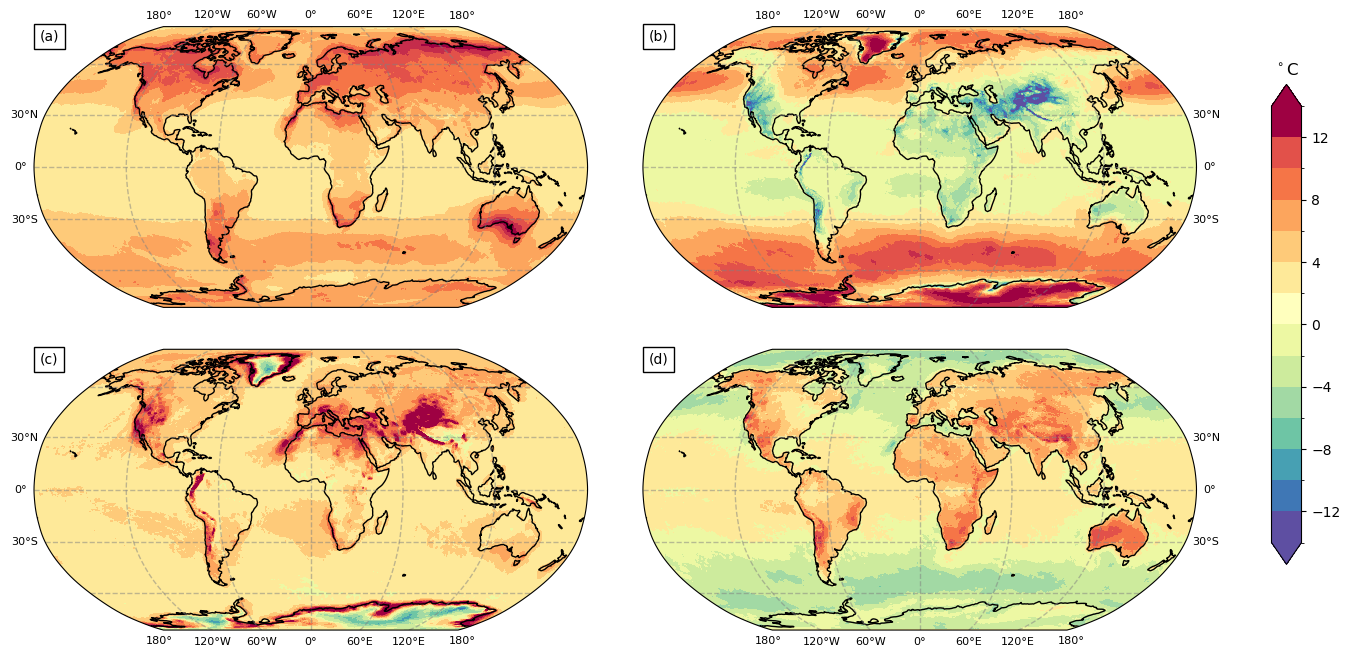
\includegraphics[width=1\linewidth]{images/mean_contribution} \caption{Reproduced from Rothlisberger and Papritz (2023). Maps at every location the mean over yearly maxima TX1day events of (a) the temperature anomaly and the anomaly contribution from (b) advective, (c) adiabatic and (d) diabatic processes.}\label{fig:decompmean}
\end{figure}

\section{Variability of hot extreme events}\label{variability-of-hot-extreme-events}

So far, we have focused on the understanding of diverse mechanisms that yield hot extreme events across the globe. Several studies have however focused on relating the variability of these processes to the resulting hot extremes variability. In the European mid-latitudes, changes in variability have been attributed to an increase in anticyclonic activity and advective heating (Lenderink et al., 2007; Horton et al., 2015; Holmes et al., 2016) and to the local effects of soil-moisture (Quesada et al., 2012; Whan et al., 2015; Donat et al., 2017; Vogel et al., 2017). Wang et al.~(2023) drew similar conclusions for Asian mid-latitudes, further relating anti-cyclonic activity increases to the North Atlantic Oscillation.

The distribution of regional-to-global hot extremes is expected to both shift positively in the mean and undergo changes in variability due to climate change (Lewis and King, 2017; McKinnon et al., 2017; R. Slater et al., 2021; E. Fischer et al.~2021; V. Thompson et al., 2022). Simolo and Corti (2022) indeed suggest that daily temperature variability changes are more important than the observed warming trend in explaining amplifications in the majority of identified hotspot regions. In an attempt to relate these changes to changes in dynamics, E. Fischer and C. Schar (2008) quantified the projected changes in hot extreme variability over Europe with respect to the processes associated with inter-annual variability, intra-seasonal variability and the seasonal variability in summer months, finding the largest contribution from the former. Di Luca et al.~(2020) quantified the contributions of annual and diurnal first and second-moment features to daily hot extremes over land, showing a diversity of global patterns. L. Suarez-Gutierrez et al.~(2020) suggests instead investigating variability changes with regard to dynamical and thermodynamical sources in European mid-latitudes, and concludes that the former - encompassing effects of atmospheric blocking - is the main driver of hot extreme variability. However, these approaches lack a direct interpretation since the temporal features may be associated with different physical processes in different regions.

\section{Methods in hot extreme literature}\label{methods-in-hot-extreme-literature}

The weather extremes literature uses two main methodologies: sensitivity and trajectory analysis. To motivate the following work, we give a brief overview of these approaches, and include Figure X to illustrate their differences.

\textbf{Sensitivity analysis} (SA) is the most widely adopted approach to study the effects of initial conditions and model parameters on outputs of a system. It involves running different experiments with simulation tools (including numerical and data-driven models) and assessing the changes in distribution of the response. Formally, sensitivity is defined as the partial derivative of the response with regard to a predictor of interest. It is then related to causality: if one assumes a linear structural model, sensitivity is a measure of the causal effect of a variable on the response. SA literature has considered both local and global measures of sensitivity. The former involves evaluating the sensitivity at a given predictor value and therefore cannot conclude general causal relationships without strong assumptions. The latter presents a difficult problem and different approaches have been proposed that include many typical statistical estimators (Razavi and Gupta, 2015).

\textbf{Trajectory analysis} (TA) follows the changes to air parcels along their flow within a dynamical system. This approach takes a Lagrangian perspective, as opposed to the Eulerian perspective that trackes changes to a volume of air at a fixed spatial coordinate. In the context of extreme weather, TA often involves the identification of an event within a numerical model followed by calculation of the flow backwards in time. The output is a timeseries of physical and model quantities that describe the state history of the parcel which gave rise to the extreme event. These characteristics have been used both to understand single events in case-studies (e.g.~Stohl and James, 2004; Huang and Cui, 2015; Papritz and Rothlisberger, 2023) as well as to gain a general understanding of drivers of extreme weather by aggregation of multiple events (e.g.~Bieli et al., 2014; Quinting and Reeder, 2017; Rothlisberger and Papritz, 2023).

This thesis uses TA to focus on process understanding of hot extreme development and will expand existing literature, introduced below.

\section{Temperature anomaly decomposition}\label{temperature-anomaly-decomposition}

This investigation is based on a Lagrangian decomposition of temperature anomaly (Rothlisberger and Papritz, 2023), which quantifies the contributions of advective (adv), adiabatic (adiab) and diabatic (diab) processes in the generation of temperature anomaly (\(T'\)). TA based on T's, rather than temperature, leads to a more natural interpretation of the components' contributions, since some processes of interest, such as warming from horizontal advection, arize due to the presence of anomalously air within a dynamic environment.

At location \(\mathbf{x}\) and starting time of the backward trajectory \(t_X\), \(T'\) may be decomposed as follows:

\begin{equation}
\begin{alignedat}{2}
   T'(\mathbf{x},t_X) = & - \int_{t_g}^{t_X} \frac{\partial \bar{T}}{\partial t} \, \text{d}\tau && \qquad \text{seas} \\
   & - \int_{t_g}^{t_X} \mathbf{\nu} \mathbf{\nabla}_h \bar{T} \, \text{d}\tau && \qquad \text{adv} \\
   & + \int_{t_g}^{t_X} \left[ \frac{\kappa T}{p} - \frac{\partial +  \bar{T}}{\partial p}\right] \omega \, \text{d}\tau && \qquad \text{adiab} \\
   & + \int_{t_g}^{t_X} \left( \frac{p}{p_0} \right)^\kappa \frac{\text{D}\theta}{\text{D}t} \, \text{d}\tau && \qquad \text{diab}
\end{alignedat}
\label{eq:tdecomp}
\end{equation}

where \(\bar{T}\) the temperature climatology; \(t_g < t_X\) genesis time, the time at which \(T'\) was last zero; \(\mathbf{\nu}\) the horizontal wind velocity; \(\mathbf{\nabla}_h\) the horizontal temperature gradient; \(p\) pressure; \(\omega\) vertical velocity; \(\theta\) potential temperature.

To study hot extremes globally and systematically, Rothlisberger and Papritz (2023) applied \eqref{eq:tdecomp} to yearly maxima of 1-day temperature anomaly averages - denoted TX1day - at every grid point in ERA5 (further described in \hyperref[data]{Data}). Timeseries of backward trajectories - calculated with LAGRANTO (Sprenger and Wernli, 2015) - are numerically integrated to approximate the integrals. Since weather phenomenon might result from different flows, for yearly maxima event at each grid-point, a total of 24 backward trajectories - corresponding to near-surface trajectory starts at 10, 30, 50 hPa and the 8 daily 3-hour timesteps - are integrated and then mean-aggregated. Each backward trajectory was back-computed until genesis \(t=t_g\) up to a maximum of 120 time-steps (15 days).

\section{Conclusion}\label{conclusion}

Although a good general understanding of mean-state hot extreme evolution exists and more detailed assessments have been made regionally and comparing specific high-impact events, a knowledge-gap in quantifying the contribution of known physical processes to hot extreme magnitude variability globally exists. This thesis attempts to close this gap by first proposing a systematic analysis of second-moment characteristics of hot extreme events and second applying state-of-the-art deep-learning methods to uncover patterns in trajectory features important for the development of hot extremes.

\chapter{Statistical Background}\label{statistical-background}

\section{Variance}\label{variance}

Variance is a measure of dispersion - or spread - of a distribution and is defined as the expected squared deviation from the mean. Given random variable \(X \sim \mathcal{F}\), the variance of \(X\) is given by \(\mathbb{V}[X] = \mathbb{E}\left[ (X-\mathbb{E}[X])^2 \right]\). Conversely to the expectation, variance is a non-linear operator. Given two random variables \(X \sim \mathcal{F}_X\) and \(Y \sim \mathcal{F}_Y\):
\begin{equation}
\begin{aligned}
\mathbb{V}[X+Y] & = \mathbb{E}\left[ (X+Y - \mathbb{E}[X+Y])^2\right] \\
& = \mathbb{E} \left[ (X - \mathbb{E}[X])^2\right] + \mathbb{E} \left[ (Y - \mathbb{E}[Y])^2\right] + 2 \, \mathbb{E}\left[ (X - \mathbb{E}[X])(Y-\mathbb{E}[Y]) \right] \\
& = \mathbb{V}[X] + \mathbb{V}[Y] + 2 \, \mathbb{C}\text{ov}[X,Y]
\end{aligned}
\label{eq:vardef}
\end{equation}

by linearity of the expectation. The last term is called the covariance between \(X\) and \(Y\) and is a measure of linear association between two random variables. Trivially, the covariance between \(X\) and \(X\) is the variance of \(X\).

These quantities serve as the basis for most statistical models. Normalizing covariance by the square-root of the variance of \(X\) and \(Y\) yields the Pearson correlation coefficient \(\rho_{X,Y}\) that is often preferred as a summary measure of linear association since it can be compared between random variables with different scales. In regression, other common measure of association between the response \(Y\) and one or more predictors \(X_{1:k}\) includes the coefficient of determination \(R^2\) measuring the proportion of the variance of \(Y\) that is predicted by \(X_{1:k}\).

In practice, one often assumed that observed data samples \(\{(x_{1},y_{1}),...,(x_n,y_n)\}\) are independent draws from some joint distribution. Then, assuming that the mean and covariance of the distribution are finite, the following provide the sample estimates of the variance of the marginal distributions \(\hat{\mathbb{V}}\) and the covariance of the joint distribution \(\hat{\mathbb{C}\text{ov}}\):

\begin{equation}
\begin{aligned}
\hat{\mathbb{V}}[\{x_{1:n}\}] &= \frac{1}{n-1} \sum_{i=1}^n \left( x_i - \bar{x} \right)^2 \\
\hat{\mathbb{C}\text{ov}}[\{x_{1:n}\},\{y_{1:n}\}] &= \frac{1}{n-1} \sum_{i=1}^n ( x_i - \bar{x})(y_i - \bar{y})
\end{aligned}
\label{eq:samplevar}
\end{equation}

where \(\bar{x} = \frac{1}{n} \sum_{i=1}^{n} x_i\) is the sample mean of \(X\). Note the normalizing factor \(n-1\) that ensures the estimate is unbiased - in repeated sampling, the average estimates equal the true quantity.

\section{Predictor importance}\label{predictor-importance}

The question of how to rank the influence a certain predictor on a response compared to other predictors is a common. Although \(R^2\) is often reported to provide comparisons of model fit and thus measure the value of certain predictors in explaining the variance of the response, it does not take into account interactions between predictors. Instead, in the context of linear regression models, Lindeman, Merenda and Gold (1980) - referred to as LMG - propose to quantify predictor importance by computing the average sequential sums-of-squares over all predictor orderings. Averaging over all orderings allows this measure to capture both direct effects and secondary effects of a predictor. Feldman (2005) extended this approach with Proportional Marginal Variance Decomposition (PMVD) that instead considers a weighted average with weights chosen to enforce the exclusion criteria - a predictor with zero coefficient is allocated zero importance (Gromping, 2007). Breiman (2001), and extensions thereof, instead propose to measure importance of a predictor by assessing the model's loss of accuracy due to random permutations of the predictor values.

This methods have however been shown to be susceptible to data with highly correlated predictors, as is often the case in observational settings lacking causal assumptions. Furthermore, with many predictors, LMG and PMVD become computationally intensive, as they require computation of R2 values over all possible orderings. Permutation-based methods scale linearly with the number of predictors but may require running many permutations of each column to output estimates with low variance.

\section{Deep Learning}\label{deep-learning}

Machine learning and in particular deep learning (DL) architectures have recently received a lot of attention in atmospheric and climate sciences due to their performance in modelling complex high-dimensional systems and their computational efficiency in comparison to numerical weather prediction. DL models have largely been used to develop weather forecasting models (see for example Srivastava and S, 2022) and to learn parameterizations from simulated and observational datasets (Barahona et al., 2023). Here, I provide a brief introduction to a DL architecture that has been used extensively in timeseries applications.

Supervised DL involves the parameterization of arbitrarily complex functions - called networks - and estimation of these parameters by propagating input data through the network and evaluating the outputs' accuracy against the given truth - called the loss. By using a differentiable loss and network, the parameters can be updated. With sufficient data and learning iterations, the parameters will be progressively updated to improve accuracy.

The modelling and processing of sequential data requires specific architectures such as Recurrent Neural Networks (RNNs) that can leverage dependencies. Long Short-Term Memory (LSTM) models are a type of RNN that were introduced by Hochreiter and Schmidhuber (1997) to solve the problem of vanishing gradients - when parameter updates become zero due to decreasing gradient magnitudes - in applications with long-term temporal dependencies. An LSTM layer is composed of a number of units, each composed of three nodes called gates: the input, forget and output gates. Given a sequence of data, each unit recurrently propagates a data sequence one timestep at a time to update the gate parameters and layer parameters that store temporal information: the hidden states that are used to communicate information from one timestep to the next, and cell states that retain a memory of the sequence characteristics. More explicitly, given initial hidden \(H_{t-1}\) and cell states \(C_{t-1}\), an input \(x_t\) at time-step \(t\) is processed in the following way:

\begin{equation}
  \begin{aligned}
    k_t &= \sigma \left( W_k \cdot [H_{t-1}, x_t] + b_k \right) \\
    l_t &= \sigma \left( W_l \cdot [H_{t-1}, x_t] + b_l\right) \\
    \tilde{C}_t &= \tanh \left( W_{\tilde{C}} \cdot [ H_{t-1}, x_t ] + b_{\tilde{C}}\right) \\
    C_t &= k_t \ast C_{t-1} + l_{t} \ast \tilde{C}_t \\
    m_t &= \sigma \left( W_m \cdot [H_{t-1}, x_t] + b_m\right) \\
    H_t &= m_t \ast \tanh (C_t)
  \end{aligned}
\label{eq:lstm}
\end{equation}

where \(\sigma\) and \(\tanh\) are the sigma and tanh activation functions; \(W_i\) and \(b_i\) are matrices of gate parameters; \(k_t,l_t\) and \(m_t\) are the outputs of the forget, input and output gates respectively. A schematic representation of this process can be found in Figure \ref{fig:lstm}.

\begin{figure}[h]

{\centering 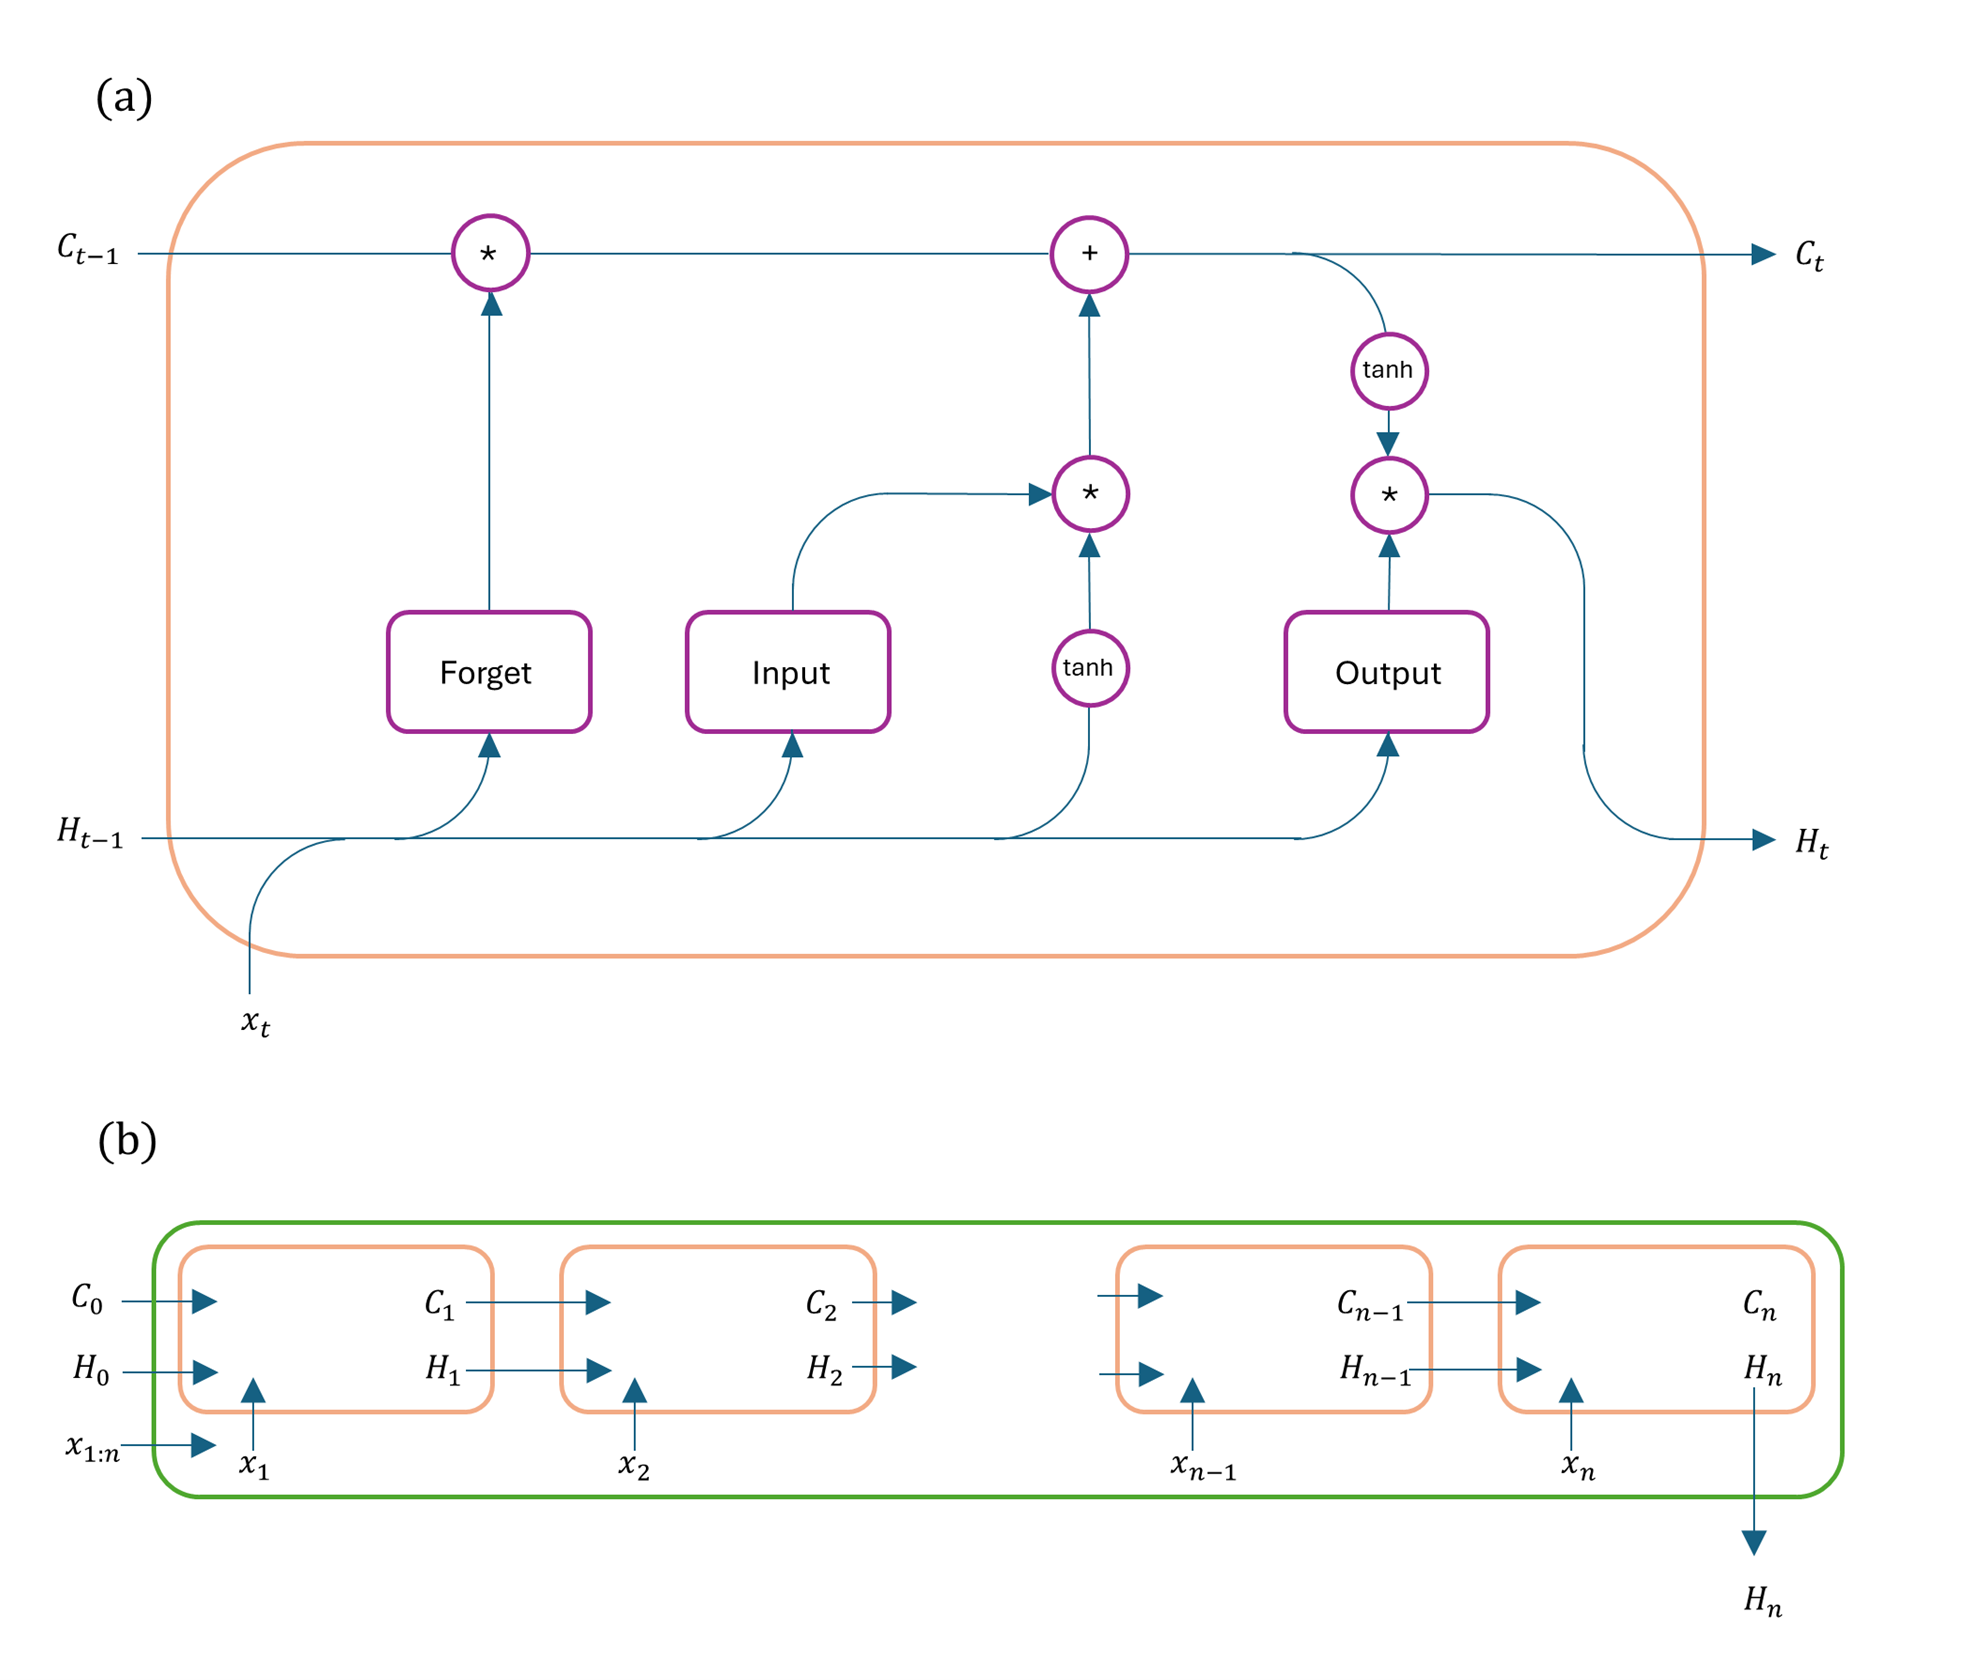
\includegraphics[width=0.8\linewidth]{images/lstm_fig} 

}

\caption{(a) Representation of an LSTM cell (in orange) that, given intitial hidden states $H_{t-1}$, cell states $C_{t-1}$ and an input $x_t$ outputs the updated hidden $H_{t}$ and cell $C_{t}$ states. Purple shapes represents operations: $\ast$ matrix multiplication, $+$ element-wise addition, tanh the activation function, and the Forget, Input and Output gates are as define in equations 3.3. (b) The same LSTM cell but unfolded. For an input of initial hidden states $H_{0}$, cell states $C_{0}$ and data sequence $x_{1:n}$, it outputs hidden states $H_t$ that can then be further processed (e.g. by a fully connected layer).}\label{fig:lstm}
\end{figure}

LSTM layers may used in different ways depending on the data structure and task at hand. In timeseries forecasting applications, most models use the final hidden states \(H_t\) of one or two LSTM layers for every input as lower-dimensional feature representations that are then further processed by one or more fully-connected NN layers. There is a rich and evolving literature on LSTM-based architectures and LSTM variants and I refer the reader to comprehensive review papers such as Hu et al.~(2020) and Han et al.~(2021).

\chapter{Data}\label{data}

\section{ERA5 and trajectory calculations}\label{era5-and-trajectory-calculations}

We apply the aforementioned methodologies to the latest ERA5 data with \(0.5^{\circ} \times 0.5^{\circ}\) horizontal resolution, 137 vertical coordinates expressed as model-levels and 3-hourly temporal resolution from 1980 to 2020. ERA5 data is model output that has been assimilated with observation and therefore represents the most complete global product of gridded meteorological data. Near-surface temperature is represented by 2m temperature and \(T'\) is calculated using transient climatologies of 9-year centered windows of 21-day periods, at every model-level. A complete description of ERA5 products may be found in Hersbach et al.~(2020).

This thesis considers the final dataset in two ways: the first section will analyse the final decomposition of each TX1day event, while the second will analyse the timeseries that evolves when considering at each backward trajectory timestep the cumulative decomposition from genesis.

\section{Final decomposition}\label{final-decomposition}

The former may be considered as a budget since it represents the total T' accumulated over its trajectory. This yields an observational dataset containing - at every {[}latitude, longitude, year{]} index - the achieved T' magnitude and the three contributors corresponding to T' gained through advective, adiabatic and diabatic processes. Numerical residuals in \eqref{eq:tdecomp} due to finite difference approximations of a continuous temporal domain are usually small and thus ignored in future analysis. Furthermore, I assume that at a location {[}latitude, longitude{]}, yearly samples are unaffected by local long-term temporal dependencies. Thus, for each location, the data consists in 41 independent draws from some multivariate distribution:

\[(T',\text{adv},\text{adiab},\text{diab}) \sim F \]
Initial exploration of the final decomposition shows a wide variety of marginal distributional behaviors, both for \(T'\) and each contributors. Figure X shows locations with right-, left-skewed and bi-modal sample histograms as well as the non-linear and highly negatively correlated relationships between contributors and with \(T'\).

\begin{figure}[h]
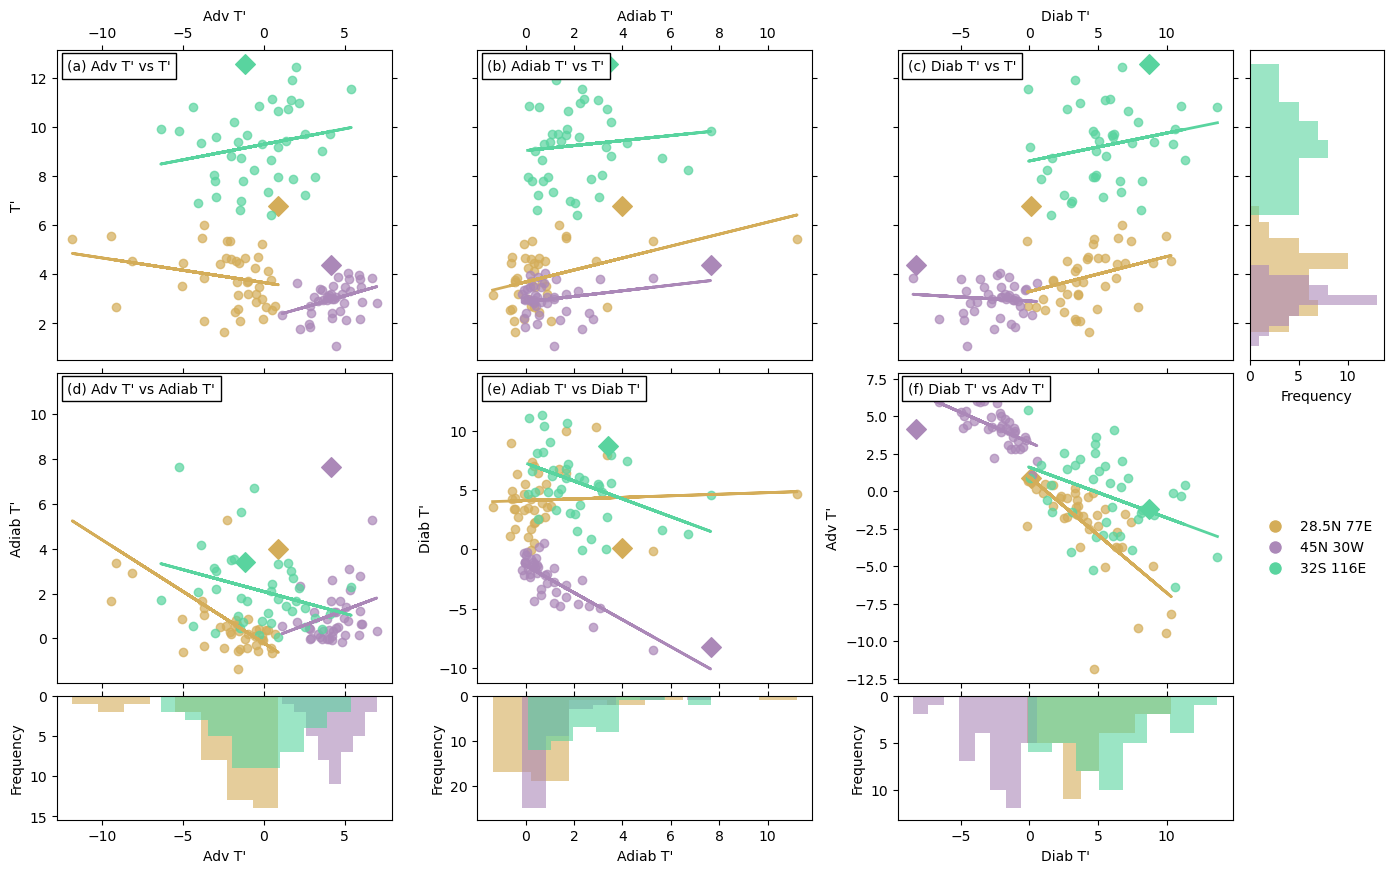
\includegraphics[width=1\linewidth]{images/flat_data} \caption{(a-c) Plots of TX1day T' against the three contributors and (e-f) pair-plots for the contributors for years 1980 to 2020 for three locations. The T' histogram is plotted on the top-right of the figure, and the contributor histograms with 8 bins are plotted below (e-f). The TX1day event acheiving largest T' is plotted as a diamond.}\label{fig:flatdata}
\end{figure}

\section{Trajectory timeseries}\label{trajectory-timeseries}

At every {[}latitude, longitude, year{]} index, the second dataset considers the time-cumulative evolution of the parcel's T', decomposed into the three contributors. Since each event may have a different genesis-time, all series are padded with zeros before their genesis time, yielding at each location 41 timeseries of length 121. The data displays again diverse structures, year-to-year as well as across space. Figure \ref{fig:timeseriesdata} illustrates the year-to-year variability for one example. T' and the contributor T's all exhibit significant positive auto-correlations, decreasing at larger time-lags. The cross-correlation between T' and the contributor T's is also large. Furthermore, the graphs show some trajectories coupling and decoupling in time: for example, the largest TX1day T' event exhibits advective and diabatic T' both decreasing until about 2 days before the event, then the diabatic T' steeply increases while the advective T' continues to decrease after a brief increase. The same pattern is observed between adiabatic and diabtic T's - although with negative correlation - up to 2 days before and then only little association.

\begin{figure}[h]
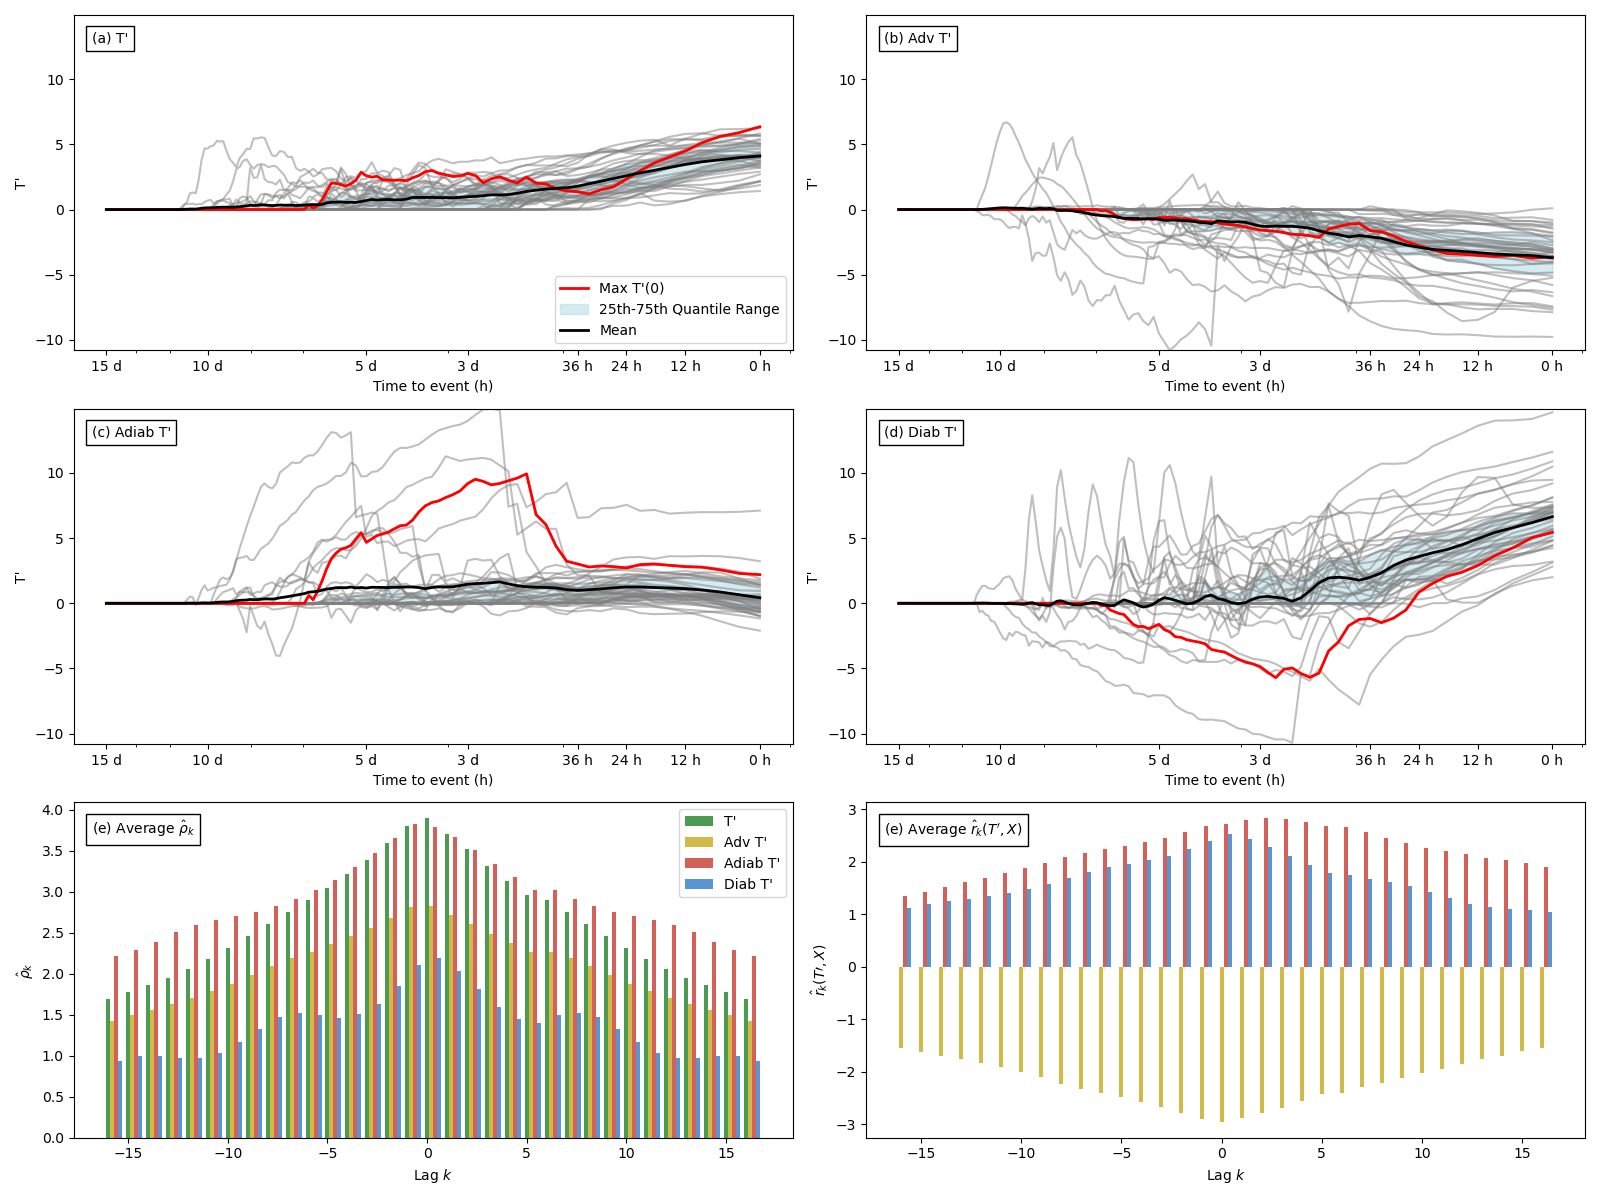
\includegraphics[width=1\linewidth]{images/timeseries_data} \caption{(a-d) Plots of TX1day T' decompositions at 16$^{\circ}$S, 48$^{\circ}$W (vicinity of Brazilia, Brazil) for years 1980 to 2020. The x-axis is logarithmic to better represent the recent history. The trajectory yielding the largest final T' among all years is colored red, the time-mean of all trajectories in black and the inter-quantile range is highlighted in light blue. The average auto-correlation (e) and cross-correlation with T' (f) over all events for each contributor. The auto- and cross-correlation are computed for timeseries starting at genesis (ignoring padding) and timeseries that are smaller than 32 timesteps are not included in the averages for lags larger than their length.}\label{fig:timeseriesdata}
\end{figure}

\chapter{Methods}\label{methods}

\section{Decomposition of TX1day anomalies and their yearly variance}\label{decomposition-of-tx1day-anomalies-and-their-yearly-variance}

The aim of this thesis is to gain further understanding in the influence of the three \(T'\)-generating mechanisms on TX1day events, particularly relating to the variability in yearly maxima observations. Then, to extend the first-moment characterization of TX1day events by M. Rothlisberger and L. Papritz (2023), we propose a variance decomposition of \(T'\) that quantifies the contributions of physical processes on variability.

Recalling \eqref{eq:tdecomp}, the evaluation of the integrals involves two errors arising from discrete approximations of the continuous time domain: error 1 denotes the deviation from zero of \(T'(\cdot ,t_g)\); error 2 denotes the remainder of the components, seasonality and error 1 subtracted from \(T'\). These errors are usually small relative to hot extreme \(T'\) magnitudes and are thus dropped in the proposed decomposition. In addition, since TX1day events evolve on sub-seasonal timescales, the seasonality term (seas) is small and is also dropped (see Extended Data in Rothlisberger and Papritz (2023)).

Then, for \(n\) temperature anomaly samples \(\{ T' \}_{1:n}\) assuming that \({T'}_i = \text{adv}_i +\text{adiab}_i +\text{diab}_i\), we have that:

\begin{equation}
   V(\{ T' \}_{1:n}) = \sum_{c \in \{\text{adv},\text{adiab},\text{diab}\}} V(\{ c \}_{1:n} ) + \sum_{c, d \in \{\text{adv},\text{adiab},\text{diab}\} , c\neq d} \text{Cov}(\{ c \}_{1:n} ,\{ d \}_{1:n})
\label{eq:vardecomp}
\end{equation}

Applying \eqref{eq:vardecomp} to every location on Earth yields a direct and systematic approach to the analysis of global patterns of hot extreme variability in the presence of complex dependencies between physical processes. The linearity of the covariance operator and the fact that it is un-normalized, in comparison to correlation for instance, allows for an intuitive comparison of second-moment contributions. I argue that considering the variance of the contributors without adjusting for the influence of other contributors due to existing correlation is more informative. For example, a large variation in adiabatic \(T'\) contribution is important to report, regardless of the additional influence of advective and diabatic processes; if the sum of adiabatic and advective \(T'\) has small variance, it will be reflected in a large negative covariance between the contributors. The limitation of using an un-normalized quantity is the fact that a large mean magnitude will in most cases imply a larger variance. Therefore, meaningful interpretation of second-moment estimates will also require consideration of first-moment estimates.

To summarize the spatial structure of TX1day \(T'\) variance and its decomposition, variance terms will be ranked with respect to their magnitude according to the following definition (applied to both mean and variance decomposition data): a contributor is dominant if it is at least twice as large as the second largest contributor; two contributors are dominant if they are both at least twice as large as the remaining contributor; else, no contributor is dominant. As both meand and variance decompositions are additive, this importance definition allows for a intuitive comparison.

Given the rich literature in feature importance (see {[}{]}), the decision to use \eqref{eq:vardecomp} is motivate by the non-trivial data structure (see \hyperref[data]{Data}). By assuming residuals to be zero, the response and predictors are linearly dependent - in addition to strong negative correlations between contributors due to inherent physical constraints. This then limits the applicability of standard regression methods and the associated measures of predictor importance that assume them uncorrelated (Hooker et al., 2021). Addressing the constraint that the response is the sum of the three contributors, for example by transforming the contributors to a simplex space (Greenacre, 2021), is also problematic as the data does not follow the positivity constraint: contributions to T' may be negative. Pre-processing the data to enforce positivity leads to poor representation of the domain and hinders interpretation. Furthermore, we do not propose more robust scale measures - such as truncated variance - in order to preserve information about tail events that are often associated with the largest human impact.

\section{Principle Component Analysis}\label{principle-component-analysis}

Strong inter-contributor correlations limit the interpretability of the above method, but are important in understanding the physical mechanisms associated with hot extreme development and their constraints. To characterize the dependence between the contributors, I employ a standard dimension reduction methodology. Principle Component Analysis (PCA), known as Empirical Orthogonal Functions in climate sciences, is a linear transformation introduced by Pearson (1901) and first applied in climate sciences for weather prediction by Lorenz (1956). Given multivariate samples of dimension \(p\), it expresses data into \(p\) orthogonal linear combinations of the original coordinates, determined iteratively to maximize variance. It is commonly used as a dimension reduction method by truncating to coordinates with high explained variance and in machine learning to yield data with uncorrelated features.

Similar to the variance decomposition, PCA is applied to the 41 samples of advective, adiabatic and diabatic T' contributions at every location on Earth. This aims to provide insights in the spatial variability of contributor dependence structures. PCA is preferred over machine-learning approaches because of the small sample sizes at each location, it is variance-based and therefore can be related to previous work, and has a intuitive interpretation.

\section{Forecasting TX1day trajectories}\label{forecasting-tx1day-trajectories}

Trajectory-based analyses for hot extreme research are often carried out case-by-case. I propose leveraging the flexibility of DL models to investigate the predictability of yearly maxima TX1day decomposition trajectories. A global LSTM-based DL model is trained to forecast the final 8 timesteps (1 day) of each component of the TX1day event decomposition trajectories given the first 112 timesteps. The model is composed of a single LSTM layer followed by a fully-connected linear layer yielding 24 outputs (3 variables x 8 timesteps) and trained via gradient descent with the mean-squared error (MSE) loss and the Adam algorithm (Kingma and Ba, 2014). Since LSTMs are known to be flexible models prone to over-fitting, L2-regularization - which penalizes the magnitude of model weights - is a common method to limit over-fitting and promote model generalization, particularly beneficial for prediction tasks on multivariate time series (Zhou et al., 2019). Given network output \(\mathbf{\hat{y}} = (\mathbf{\hat{y}}_{\text{adv}}, \mathbf{\hat{y}}_{\text{adiab}}, \mathbf{\hat{y}}_{\text{diab}})\) and truth \(\mathbf{y} = (\mathbf{y}_{\text{adv}}, \mathbf{y}_{\text{adiab}}, \mathbf{y}_{\text{diab}})\), model parameters \(\mathbf{W}\) and some weight hyperparameter \(r\), the objective function is given by:

\begin{equation}
   \text{obj}(\mathbf{\hat{y}},\mathbf{y}) = \frac{1}{24}\sum_{i=1}^{24} (y_i - \hat{y}_i)^2 + r \cdot || \mathbf{W} ||_2 
\label{eq:obj}
\end{equation}

where \(||\cdot ||_2\) is the L2-norm.

Due to the high-resolution of ERA5 data and considering 40 years of data, the dataset contains over 10 million timeseries. The flattened globe is divided into 16 rectangular regions according to Figure \ref{fig:traintest}: 8 will be used for training, and 8 for validation. The timeseries exhibit large spatial dependencies within a given year since they may share the same flow. Therefore, to further promote a more general model, the validation regions are reduced in latitude and longitude extent by a factor proportional to the maximum of the average trajectory distance in each region. Furthermore, to limit computational burden and allow inference on unseen data everywhere on the globe, only years from 1980 to 2000 are used for training.

A single model instance is trained for each combination of LSTM layer hidden unit size {[}64,128,256{]} and L2-regularization weight {[}0.00001,0.0001,0.001{]} and the instance achieving the lowest objective \eqref{eq:obj} is chosen for inference. A rich model is encouraged by using a low batch-size of X on the shuffled training data and an initial learning rate of Y.

\begin{figure}[h]

{\centering 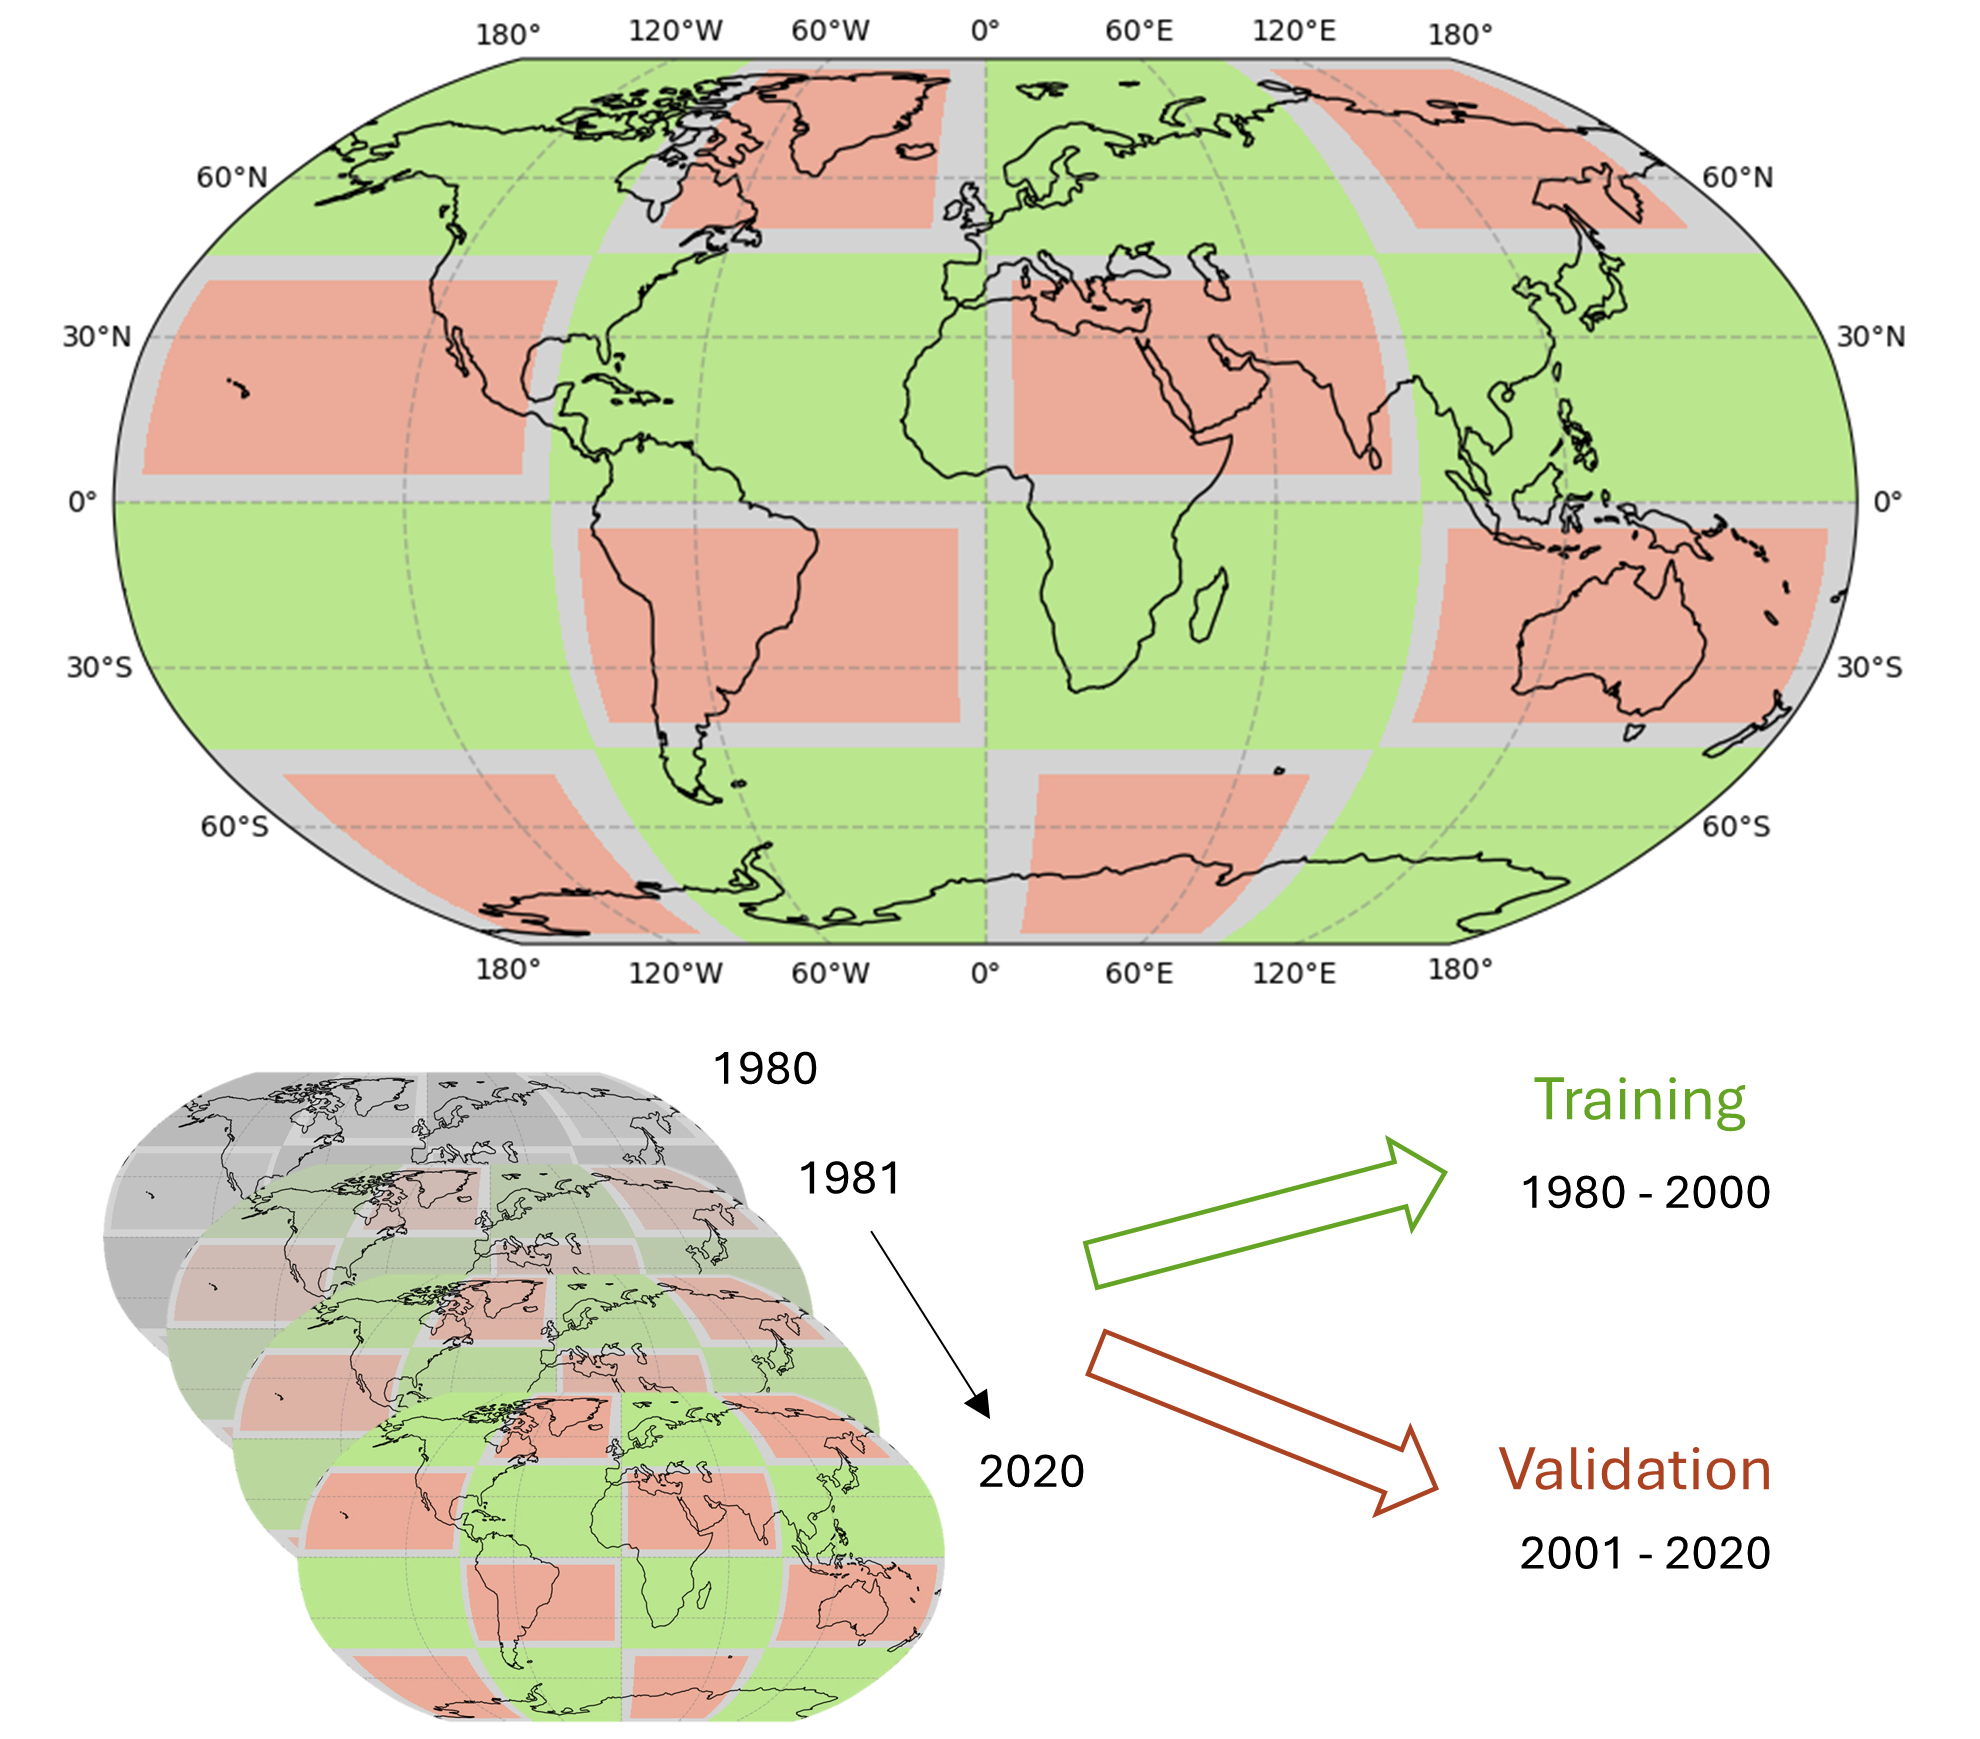
\includegraphics[width=0.9\linewidth]{images/test_train_fig} 

}

\caption{Training and validation splitting scheme. Years between 1980 and 2000 are used for training (green shaded areas) and validation (red shaded areas). The remaining years 2001 to 2020 and the whole globe are used for inference.}\label{fig:traintest}
\end{figure}

\chapter{Results}\label{results}

\section{Relating TX1day T' variability to component variability}\label{relating-tx1day-t-variability-to-component-variability}

The variance decomposition on 40 years of ERA5 data reveals large spatial diversity in year-to-year TX1day variance (Figure \ref{fig:vardecomp}). As anticipated, the patterns closely resemble those of the mean of TX1day magnitudes in Rothlisberger and Papritz (2023), since the variance is un-normalized and therefore scales with magnitude. There is a strong ocean-land contrast, with low variances in the order of 2 K\(^2\) over oceans and mostly above 4 K\(^2\) over land. A general trend over land is the increase in variability further from the Equator. There exists nonetheless important exceptions: the West coasts of North America, West coasts of Southern Chile, South-western coasts of Australia and the West coasts between Mauritania and Northern Europe all exhibit large TX1day variability, while tropical land such as the Amazonia, South-east Asia and Indonesia, equatorial Africa and parts of the Eastern Saharan show low variability compared to the oceans. The largest peaks of variability occur in the bay of the Antarctic Peninsula and an oceanic hot spot centered at 70° S 160° W, as well as relatively large hotspots in the coastal regions described above.

Individual contributors have mostly larger variance and vary spatially with no single contributor dominating globally. The advective and adiabatic \(T'\) variance have similar spatial distribution over land, while they seem to complement each other over oceans with large adiabatic \(T'\) variance in the extra-tropics and large adiabatic \(T'\) variance in the sub-tropics. Key hotspots of very large variance for both contributors include regions of high topography (particularly over Rockies, the Andes and the Himalayas) as well as the Arctic and Antarctic ice sheets, with values mostly above 32 K\(^2\) and 64 K\(^2\) respectively. In comparison, the variances of diabatic \(T'\) are more uniform with a less pronounced ocean-land contrast, and are particularly small over oceans east of the continents at the Equator with values between 0 and 2 K\(^2\). The storm track regions, especially the upstream portions of the NH, have larger advective \(T'\) variance than the surrounding oceans, which resembles the TX1day variance map.

Covariances between contributors are predominantly negative and again display diverse spatial patterns. The covariances between advective and adiabatic \(T'\) are positive only over the extra-tropical oceans; between advective and diabatic \(T'\) over small regions in the tropical oceans and the Greenland and Antarctic ice sheets; between diabatic and adiabatic \(T'\) over regions of high topography and within the African and Australian continents. Over oceans, the covariance between advective-adiabatic and advective-diabatic complement each other with positive and negative contributions, while the covariance between diabatic and adiabatic \(T'\) is almost always negative.

Spatial patterns in mean magnitude of contributors mainly agree with those in the variance over land, but not over the oceans. The advective \(T'\) patterns are most different on the coast of Western North-America, coastal North-western Africa and the ocean region West of Australia. The diabatic \(T'\) patterns are the most different, in particular over Southern hemisphere oceans, where the mean patterns show much stronger latitudinal gradient and miss important large-variance regions on the west of the continents. The adiabatic \(T'\) patterns instead shows good agreement over the oceans, while some differences exist in the Sahara, eastern North-America and the storm tracks, both in the Northern and Southern hemispheres.

\begin{figure}[h]
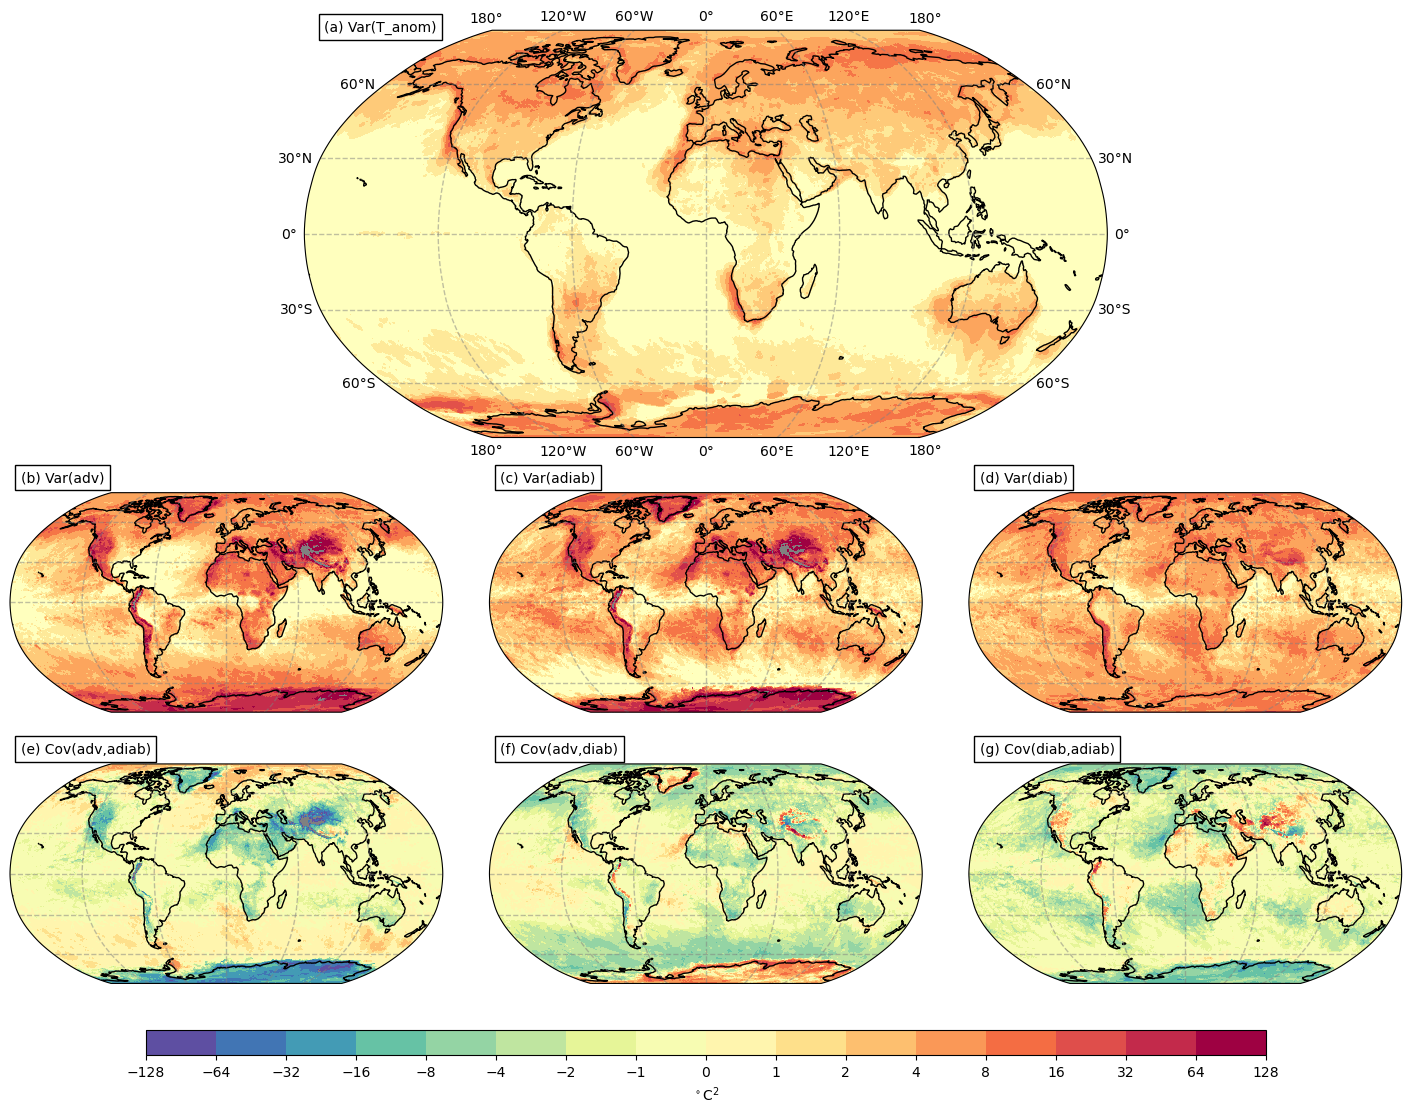
\includegraphics[width=1\linewidth]{images/vardecomp} \caption{(a) Variance of TX1day series decomposed into (b) variance of advective $T'$, (c) adiabatic $T'$, (d) diabatic $T'$, and the the covariances between the contributors (e,f,g). Grid points with very high variances or covariances magnitudes (below -128 and above 128, corresponding to less than 0.6\% of all observations) are colored grey.}\label{fig:vardecomp}
\end{figure}

Similarly to mean-characteristics, the ocean-land contrasts in TX1day variance can be explained by water's larger heat capacity, since a slower temperature gain by solar radiation limits the short-term gain in temperature of a parcel. This is supported by a more uniform diabatic \(T'\) variance over oceans and suggests that cloud cover can influence \(T'\) growth particularly at the end of TX1day event trajectories when parcels are close to the ocean surface. Regions of larger variance over oceans - in TX1day \(T'\) and all contributors - are found near the coasts and can be attributed to trajectories that predominately evolve over land and therefore involve more variable heat-generating mechanisms.

For example, the variability hotspot located on North-Western African coast involves the typical summer-time Azores high-pressure system inducing trade winds from North and the Saharan low-pressure system inducing the Harmattan winds that originate from the continent (Adame et al., 2022), converging on the Moroccan coast and travelling in a South-westerly direction along the coast. Yearly variability in this synoptic situation can then lead to changes in the contributions from trade winds or Harmattan winds, that evolve very differently.

The mean decomposition showed large cancellation between contributors in many regions. The generally large and negative covariances supports this fact. Furthermore, these regions tend to exhibit large variance in both/either/one of the contributing processes. The Northern and Southern Hemisphere storm tracks have large mean positive contributions from advective \(T'\) with large dampening by diabatic \(T'\), while small but positive contributions from advective \(T'\). This study confirms that observed variability in the TX1day \(T'\) is impacted both by variability in these competing mechanisms, but additionally finds moderate contribution from adiabatic \(T'\) and the covariance between advective and adiabtic \(T'\) in the upstream portion of the storm tracks, that has previously been neglected. This observation is also noted in Easten Brazil, continental southern Africa, Australia and the northern East coast of North America - although with diabatic \(T'\) and advective \(T'\) contributing positively and negatively in the mean, respectively. This is highly significant since changes in variability of hot extremes under climate change may not only be influenced by changes in mean-dominant physical processes, but also those that affect second-moment characteristics, supporting work by Simolo and Corti (2022).

Assessing the variability in these dampening mechanisms, or attributing importance of the positive or negative contributor, is difficult without considering the temporal evolution of these interactions. However, the spatial patterns in the covariance between the contributors is then a useful tool in determining regions where competing effects are present and influence the observed variability of resulting TX1day events. Furthermore, the diversity in covariance patterns is suggestive of complex and sensitive TX1day events.

\section{Comparing contributions to TX1day T' mean and variance}\label{comparing-contributions-to-tx1day-t-mean-and-variance}

Figure XX maps the most important contributor/s - according to to the definition introduced in \hyperref[decomposition-of-tx1day-anomalies-and-their-yearly-variance]{Methods} - for the mean (Rothlisberger and Papritz, 2023) and variance decompositions to more concisely compare their differences.

\begin{figure}[h]
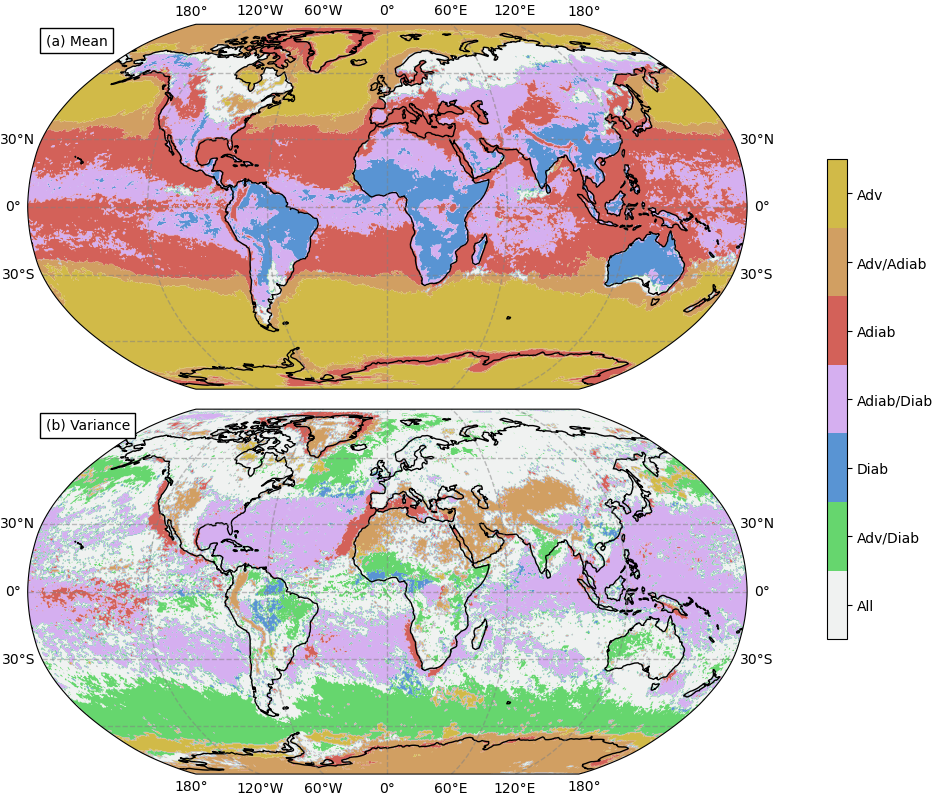
\includegraphics[width=1\linewidth]{images/dominant} \caption{(a) Reproduced from Rothlisberger and Papritz (2023). Maps at every location the most important contributor to average TX1day yearly maxima magnitude. (b) Maps at every location the most important variance term to variance of TX1day yearly maxima magnitudes. Contributor A is most important if it is 2 times larger than the second largest contributor. Contributors A and B are collectively most important if the smallest of the two is 2 times larger than the least important contributor. Else, all contributors are deemed important.}\label{fig:dominant}
\end{figure}

In most oceanic and subtropical land, advective and/or adiabatic \(T'\) dominates the mean while the variance is characterized additionally by significant contribution from diabatic \(T'\). This is highlighted in the Northern and Southern Hemisphere storm tracks. In remaining regions with mean-dominating diabatic \(T'\), the variance of TX1day \(T'\) is dominated by diabatic \(T'\) and most often advective \(T'\) - such as in Equatorial Africa, Eastern South America, Western Australia and Eastern India. In fact, only few regions have a single dominating contributor in the variance. The North-western African, South-western African and Western North-american coasts, a large part of the Mediterranean and the tropical Pacific are dominated by adiabatic processes. Small regions in the Amazonia, Western equatorial Africa and small regions south of the Northern Hemisphere storm tracks are dominated by diabatic processes. Finally, the upstream portion of the Northern Hemisphere storm tracks and a small coastal band around the Antarctic are dominated by advective processes.

Regions of high-topography, high adiabatic in mean vs additional advective influence in variance. Thoughts?

The coastal regions that showed peaks in TX1day \(T'\) variance are primarily dominated by adiabatic \(T'\) both in the variance and in the mean.

Important disagreement between the maps involve only small regions. Off the Southern-East coast of Australia, advective \(T'\) mostly dominates the mean while adiabatic and diabatic \(T'\) dominate the variance.

Although the larger influence of diabatic \(T'\) globally supports previous evidence that radiative and land surface processes dominate sub-tropical changes in summer-time near-surface temperature variability (Holmes et al., 2016), this work further highlights the importance in considering all three heat-generating mechanisms. Furthermore, over Australia, advective processes have been understood to be dominating the observed changes in summer-time near-surface temperature variability (Watterson et al., 2008; Holmes et al., 2016). This study agrees, but further insists that for hot extremes, both diabatic - dominant in the West - and adiabatic processes cannot be ignored.

Then the variance of TX1day \(T'\) is almost entirely dominated by more processes than its mean counterpart. The implications is that process understanding of hot extreme development, particularly over land, requires more careful examination of changes in the physical processes due to climate changes. In showing that less important mechanisms for mean characterization of TX1day events - such as advective processes in western Europe - become significant when quantifying year-to-year variability, this study suggests a r

\section{Inter-component variability structure}\label{inter-component-variability-structure}

The covariances discussed in \hyperref[relating-tx1day-t-variability-to-component-variability]{6.1} are useful in quantifying the importance of contributor interactions to TX1day variance, but could not provide a clear characterization of the dependence structures. To address this limitation, this section focuses only on the variability of the contributors. Applying PCA to yearly TX1day event \(T'\) decompositions at every location on Earth and examining the resulting proportion of explained variance by each component (figure @ref(fig:pca\_explainedvar)) reveals that the advective, adiabatic and diabatic \(T'\) contributions are constrained by one or two main axes of variability.

\begin{figure}[h]
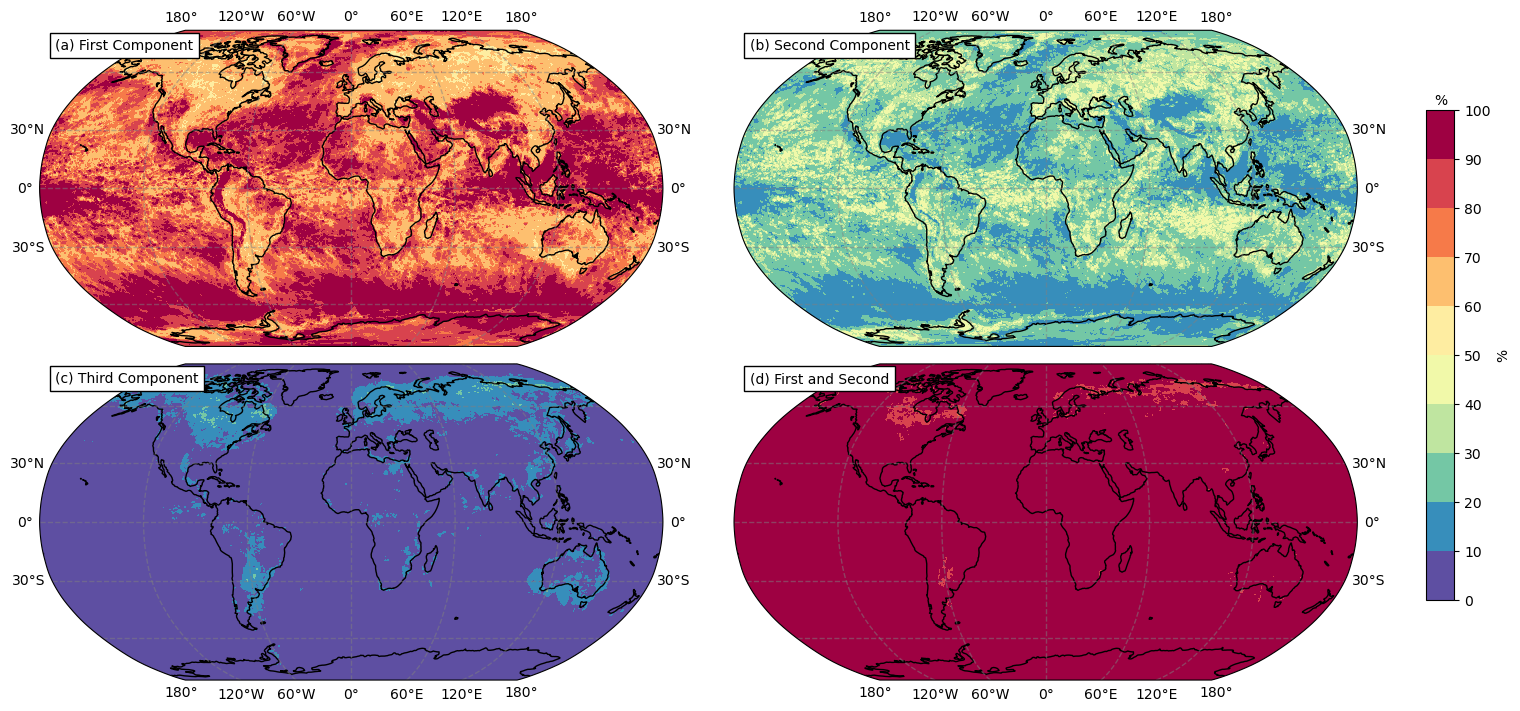
\includegraphics[width=1\linewidth]{images/pca_explainedvar} \caption{Percentage of variance in the advective, adiabatic and diabatic temperature anomaly that is explained by (a) the first PC, (b) the second PC, (c) the third PC and (d) the first and second PCs.}\label{fig:pcaexplainedvar}
\end{figure}

The central Andes and Himalayan plateaus, off the southern and eastern coast of Sri-lanka, the South China and Philippines seas as well as regions of the coast of the Antarctic have over 95\% of their variance in the contributors explained by the first PC. The regions of high topography highlighted in section \hyperref[relating-tx1day-t-variability-to-component-variability]{6.1} to have very large covariance contributions then indicate strong coupling between all three components. The tropical regions were not observed to have such structures due to the presence of relatively small TX1day \(T'\) values. This is a surprising result, as the weather in this region is modulated by diverse mechanisms including large circulation patterns induced by SST anomalies in the Pacific and Indian oceans as well as strong soil moisture - temperature feedbacks (Jiang et al., 2023).

Most of the remaining oceans, large parts of Africa and the middle East, Easter Australia, Greenland and the Antarctic, the western North-america and North-eastern South America have between 70 and 95\% of the variance explained by the first PC. This suggests that, globally, TX1day event contributor trajectories evolve under strong physical constraints. BLAH BLAH BLAH.

Then, only few regions require three PCs to explain over 85\% of the variance in the three contributors. These are almost always land areas - apart from small regions off the coast of Norway and North-western Russia.

The analysis of total contributions to TX1day \(T'\) variance of the advective, adiabatic and diabatic processes and their dependence structure is however limited since it does not consider any temporal information. Contributions from a process may occur at any point in the trajectory and the presence of cyclic processes may inflate magnitudes of the final decomposition. To more precisely attribute \ldots{}

\section{Trajectory analysis with ML}\label{trajectory-analysis-with-ml}

\section{Extras}\label{extras}

What do we want to discuss here:
* Try to explain the largest patterns that occur: land-ocean contrast, coastal hotspots, mountain and arctic hotspots, talk about European hot extremes maybe.
* Relate the findings to the literature: The paper from Laura, dampening mechanisms with the paper from Matthias, tropical lows and soil moisture effects. How does soil moisture affect the variability of hot extreme events year-to-year? One may say the variability in soil moisture is important.
* Don't re-invent the wheel: talk about the differences to mean-characteristics.

Good article to compare and/or justify patterns: Large-scale emergence of regional changes in year-to-year temperature variability by the end of the 21st century

\chapter{Discussion}\label{discussion}

Lorem ipsum dolor sit amet, consectetur adipiscing elit, sed do eiusmod tempor
incididunt ut labore et dolore magna aliqua. Ut enim ad minim veniam, quis
nostrud exercitation ullamco laboris nisi ut aliquip ex ea commodo consequat.
Duis aute irure dolor in reprehenderit in voluptate velit esse cillum dolore
eu fugiat nulla pariatur. Excepteur sint occaecat cupidatat non proident, sunt
in culpa qui officia deserunt mollit anim id est laborum

\chapter{Conclusion}\label{conclusion-1}

I expect that a successful timeseries model would be able to accomodate: a variety of different classes of multivariate behaviours which can be interpreted as general heat-generating flows; assess the influence of early-development characteristics of parcels in addition to the more important recent history; forecast all contributors 12-36 hours (4-12 timesteps) hours ahead; be able to assign importance to specific timesteps or subsequences, or output a causal graph structure for each class.

Does variability in the final TX1day magnitude originate from early development or from recent history?
%%%%%%%%%%%%%%%%%%%%%%%%%%%%%%%%%%%%%%%%%%%%%%%%%
%%% Bibliography                              %%%
%%%%%%%%%%%%%%%%%%%%%%%%%%%%%%%%%%%%%%%%%%%%%%%%%
\addtocontents{toc}{\vspace{.5\baselineskip}}
\cleardoublepage
\phantomsection

\bibliography{bib/bib}
\addcontentsline{toc}{chapter}{\bibname}

%% All books from our library (SfS) are already in a BiBTeX file
%% (Assbib). You can use Assbib combined with your personal BiBTeX file:
%% \bibliography{Myreferences,Assbib}. Of course, this will only work on
%% the computers at SfS, unless you copy the Assbib file
%%  --> /u/sfs/bib/Assbib.bib

%%%%%%%%%%%%%%%%%%%%%%%%%%%%%%%%%%%%%%%%%%%%%%%%%
%%% Appendices (if needed)                    %%%
%%%%%%%%%%%%%%%%%%%%%%%%%%%%%%%%%%%%%%%%%%%%%%%%%
\addtocontents{toc}{\vspace{.5\baselineskip}}
\appendix
\chapter{Supplementary material on timeseries data}

\section{Further examples of trajectory data}

Find below the trajectory timeseries visualisation plots - as figure 4.2 - for the locations in figure 4.1. Each figure contains plots (a-d) of TX1day T’ decompositions for years 1980 to 2020. The x-axis is logarithmic to better represent the recent
 history. The trajectory yielding the largest final T’ among all years is colored red, the
 time-mean of all trajectories in black and the inter-quantile range is highlighted in light
 blue. It also contains the average auto-correlation (e) and cross-correlation with T’ (f) over all events
 for each contributor. The auto- and cross-correlation are computed for timeseries starting
 at genesis (ignoring padding) and timeseries that are smaller than 32 timesteps are not
 included in the averages for lags larger than their length.

\begin{figure}[h]
\caption{Location 28.5N 77E, in the vicinity of New Delhi, India.}
\centering
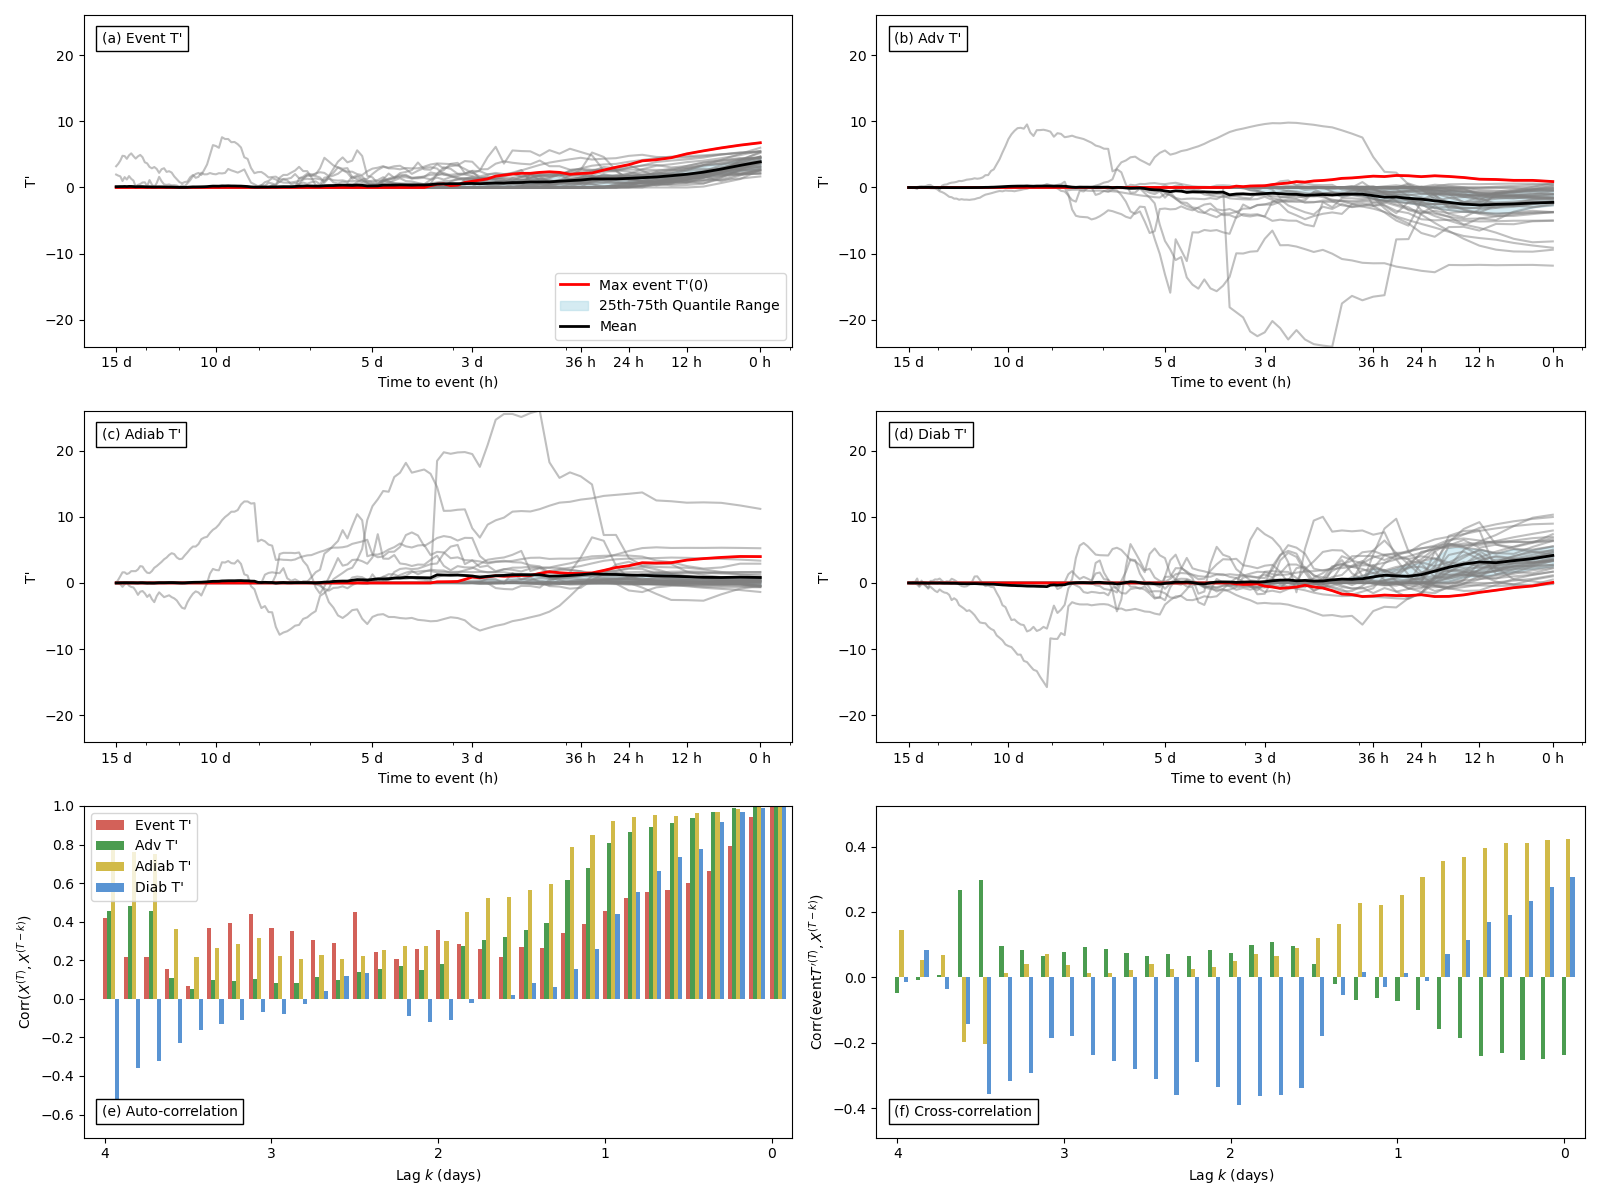
\includegraphics[width=0.9\textwidth]{images/sup1.png}
\end{figure}

\begin{figure}[h]
\caption{Location 45N 30W, in the middle of the Atlantic ocean.}
\centering
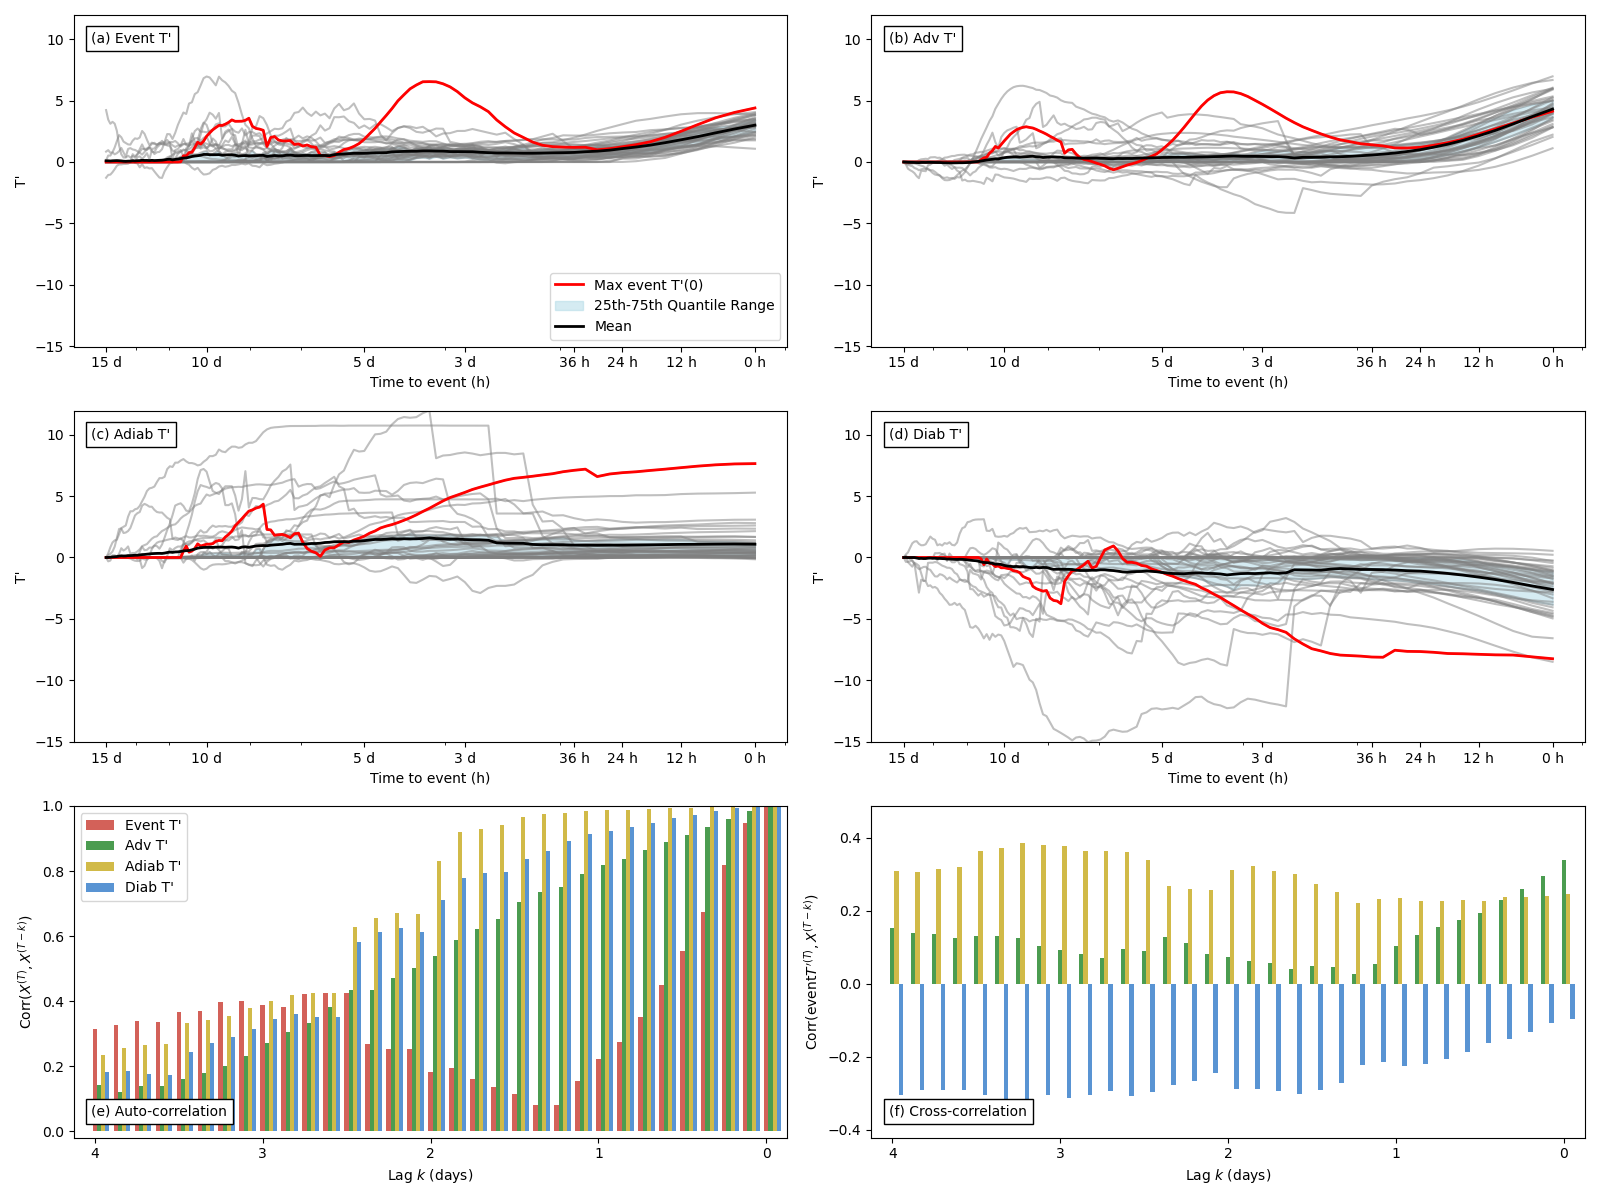
\includegraphics[width=0.9\textwidth]{images/sup2.png}
\end{figure}

\begin{figure}[h]
\caption{Location 32S 116E, in the vicinity of Perth, Australia.}
\centering
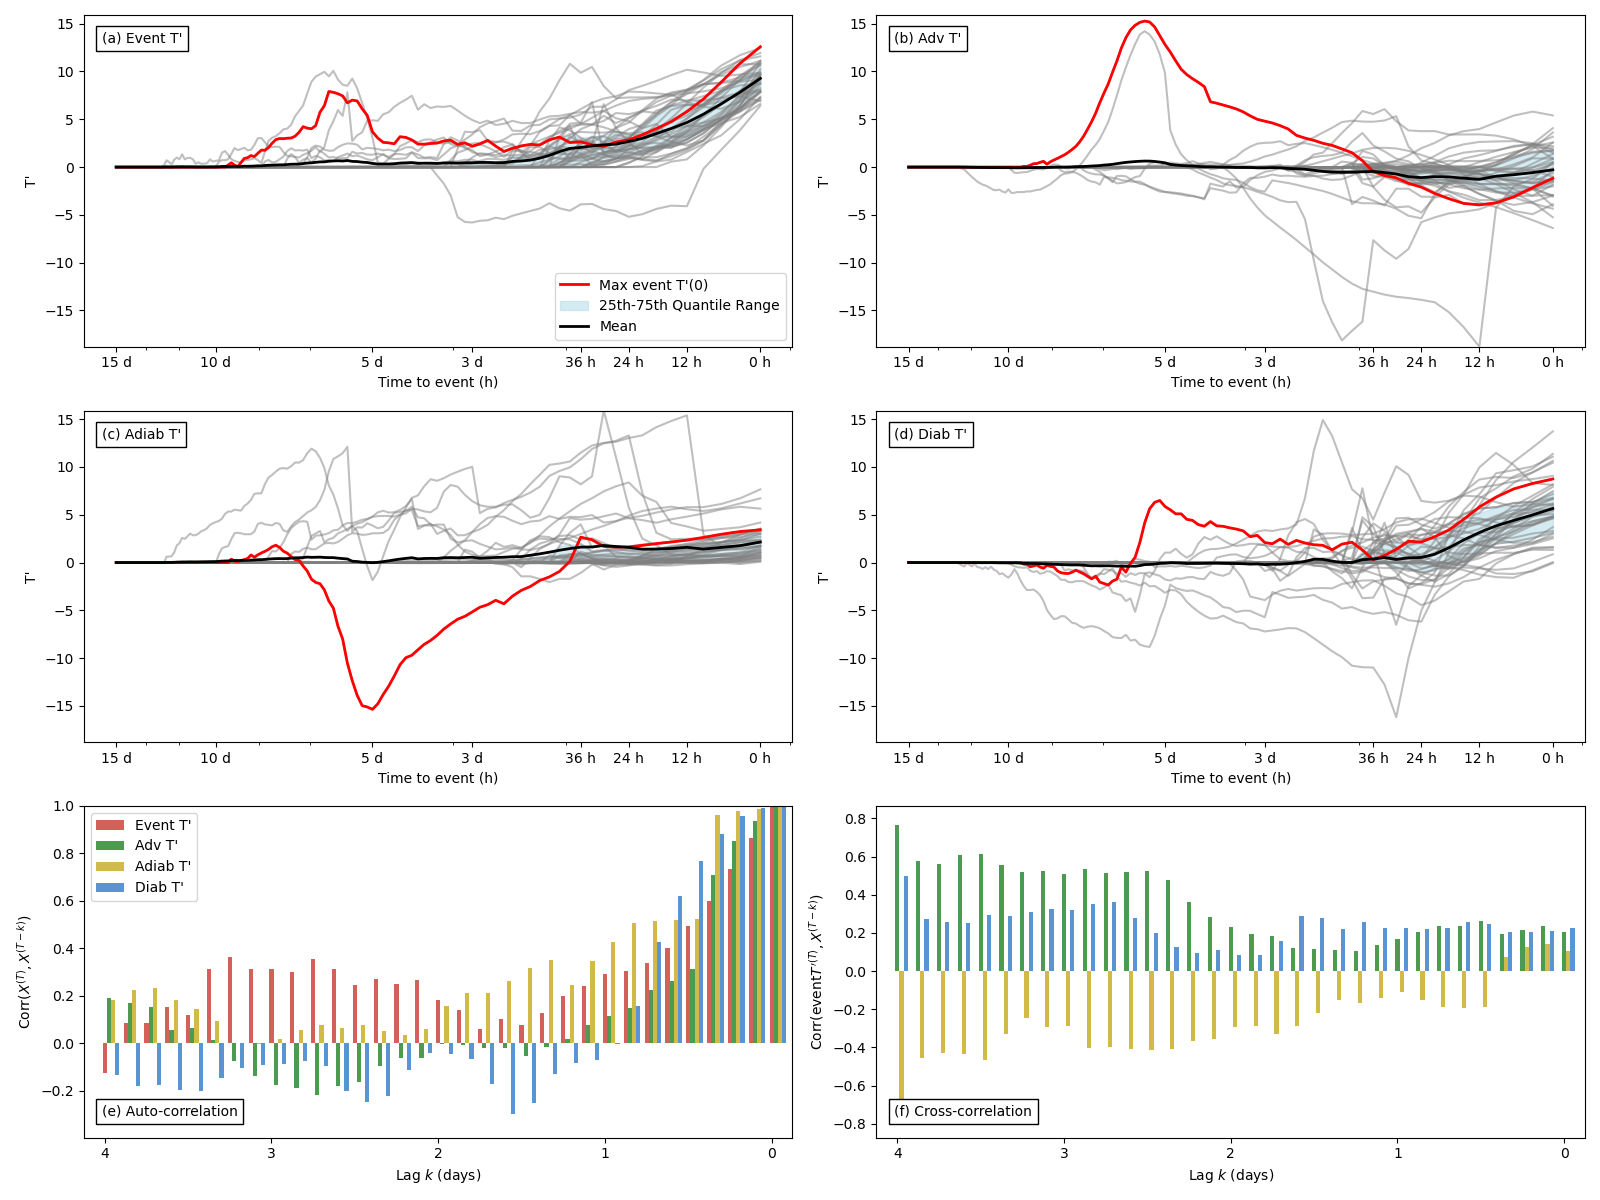
\includegraphics[width=0.9\textwidth]{images/sup3.png}
\end{figure}

\section{Differenced timeseries data}

%%% Local Variables: 
%%% mode: latex
%%% TeX-master: "MasterThesisSfS"
%%% End: 



%%%%%%%%%%%%%%%%%%%%%%%%%%%%%%%%%%%%%%%%%%%%%%%%%%
%%% Declaration of originality (Do not remove!)%%%
%%%%%%%%%%%%%%%%%%%%%%%%%%%%%%%%%%%%%%%%%%%%%%%%%%
%% Instructions:
%% -------------
%% fill in the empty document confirmation-originality.pdf electronically
%% print it out and sign it
%% scan it in again and save the scan in this directory with name
%% confirmation-originality-scan.pdf
%%
%% General info on plagiarism:
%% https://www.ethz.ch/students/en/studies/performance-assessments/plagiarism.html
\cleardoublepage

\includepdf[pages={-}, frame=true,scale=1]{pdf/confirmation-originality.pdf}
\end{document}
